%% FEUP THESIS STYLE for LaTeX2e
%% how to use feupteses (English version)
%%
%% FEUP, JCL & JCF, 31 July 2011
%%
%% PLEASE send improvements to jlopes at fe.up.pt and to jcf at fe.up.pt
%%

%%========================================
%% Commands: pdflatex tese
%%           bibtex tese
%%           makeindex tese (only if creating an index) 
%%           pdflatex tese
%%========================================

\documentclass[11pt,a4paper,twoside,openright]{report}

%% For iso-8859-1 (latin1), comment next line and uncomment the second line
\usepackage[utf8]{inputenc}
%\usepackage[latin1]{inputenc}

%% English version

%% MIEIC options
%\usepackage[mieic]{feupteses}
%\usepackage[mieic,juri]{feupteses}
\usepackage{alltt}
%\usepackage[mieic,final]{feupteses}
\usepackage[mieic,final,onpaper]{feupteses}

%% Additional options for feupteses.sty: 
%% - onpaper: links are not shown (for paper versions)

%% Uncomment the next lines if side by side graphics used
%\usepackage[lofdepth,lotdepth]{subfig}
%\usepackage{graphicx}
%\usepackage{float}

%% Include color package
\usepackage{color}
\definecolor{cloudwhite}{cmyk}{0,0,0,0.025}

%% Include source-code listings package
\usepackage{listings}
\lstset{ %
 language=C,                        % choose the language of the code
 basicstyle=\footnotesize\ttfamily,
 keywordstyle=\bfseries,
 numbers=left,                      % where to put the line-numbers
 numberstyle=\scriptsize\texttt,    % the size of the fonts that are used for the line-numbers
 stepnumber=1,                      % the step between two line-numbers. If it's 1 each line will be numbered
 numbersep=8pt,                     % how far the line-numbers are from the code
 frame=tb,
 float=htb,
 aboveskip=8mm,
 belowskip=4mm,
 backgroundcolor=\color{cloudwhite},
 showspaces=false,                  % show spaces adding particular underscores
 showstringspaces=false,            % underline spaces within strings
 showtabs=false,                    % show tabs within strings adding particular underscores
 tabsize=2,	                    % sets default tabsize to 2 spaces
 captionpos=b,                      % sets the caption-position to bottom
 breaklines=true,                   % sets automatic line breaking
 breakatwhitespace=false,           % sets if automatic breaks should only happen at whitespace
 escapeinside={\%*}{*)},            % if you want to add a comment within your code
 morekeywords={*,var,template,new}  % if you want to add more keywords to the set
}

%% Uncomment to create an index (at the end of the document)
%\makeindex

%% Path to the figures directory
%% TIP: use folder ``figures'' to keep all your figures
\graphicspath{{figures/}}

%%----------------------------------------
%% TIP: if you want to define more macros, use an external file to keep them
%some macro definitions

% format
\newcommand{\class}[1]{{\normalfont\slshape #1\/}}

% entities
\newcommand{\Feup}{Faculdade de Engenharia da Universidade do Porto}

\newcommand{\svg}{\class{SVG}}
\newcommand{\scada}{\class{SCADA}}
\newcommand{\scadadms}{\class{SCADA/DMS}}

%%----------------------------------------

%%========================================
%% Start of document
%%========================================
\begin{document}

%%----------------------------------------
%% Information about the work
%%----------------------------------------
\title{Web System For Creating And Managing Virtual High Performance Computing Environments}
\author{Pedro Adriano Pessoa Teixeira}

%% Uncomment next line for date of submission
%\thesisdate{July 31, 2008}

%%Uncomment next line for copyright text if used
%\copyrightnotice{Name of the Author, 2008}

\supervisor{Supervisor}{Jorge Manuel Gomes Barbosa}{(PhD)}

%% Uncomment next line if necessary
%\supervisor{Co-Supervisor}{Tito Carlos Soares Vieira}{(MSc)}

%% Uncomment committee stuff in the final version if used
\committeetext{Approved in oral examination by the committee:}
\committeemember{Chair}{Pedro Alexandre Guimarães Lobo Ferreira do Souto (PhD)}
\committeemember{External Examiner}{Pedro Manuel Henriques da Cunha Abreu (PhD)}
\committeemember{Supervisor}{Jorge Manuel Gomes Barbosa (PhD)}
\signature

%% Specify cover logo (in folder ``figures'')
\logo{feup-logo.pdf}

%%----------------------------------------
%% Preliminary materials
%%----------------------------------------

% remove unnecssary \include{} commands
\begin{Prolog}
  \chapter*{Abstract}

Current Grid computing infrastructures are generally not very flexible when it comes to the users' needs. As such, whenever it is required, the user must adapt its code to the infrastructures specifications.

On the other hand, Cloud Computing is associated with an extreme flexibility allowing the infrastructure to adapt itself to the users' requirements. Another aspect present in Cloud Computing but non-existent in Grid Computing is the Quality of Service factor, where a user can submit a job according to a certain cost or deadline.

FEUP --- Faculty of Engineering of Port University --- has started developing a private cloud project at its Informatics center (CICA --- Informatics Center Prof. Correia de Araújo) --- in which a user can create custom Virtual Machine images on-the-fly and have the system automatically provision the required resources to run the submitted job.

\textit{OpenStack} and \textit{OpenNebula} are competing cloud management platforms, both with their own methods of dealing with Virtual Machine images. 

In this report both cloud management platforms are reviewed in great detail and a choice is made as to which one to use in FEUP's private cloud project. The technologies that support these platforms are also discussed so that the reader can be properly contextualized.

The work and research involved in creating a web system based on \textit{Python} and \textit{Django} that is capable of creating Virtual Machine images according to the users requisites, as well as capable of registering those VM images with a cloud management platform, namely \textit{OpenStack}, is also documented.


\chapter*{Resumo}

As infraestruturas actuais de computação em Grelha geralmente não são muito flexíveis no que diz respeito às necessidades dos utilizadores. Assim sendo e sempre que é necessário, é o utilizador que tem de adaptar o código às especificações das infraestruturas.

Por outro lado, a computação em Nuvem é associada a uma flexibilidade extrema, permitindo assim que seja a estrutura a adaptar-se aos requisitos do utilizador. Outro aspecto presente neste tipo de computação, mas que é totalmente ausente na computação em Grelha, é o factor Qualidade de Serviço, em que um utilizador pode submeter um trabalho de acordo com um determinado custo ou um determinado prazo.

A FEUP --- Faculdade de Engenharia da Universidade do Porto --- começou a desenvolver o seu próprio projecto de nuvem privada no seu centro de informática (CICA --- Centro de Informática Prof. Correia de Araújo) em que um utilizador pode criar as suas imagens de máquinas virtuais \textit{on-the-fly} e ser o sistema a provisionar os recursos necessários para correr o trabalho de computação desejado.

\textit{OpenStack} e \textit{OpenNebula} são duas plataformas de gestão de nuvens, competidoras no mercado, sendo que ambas possuem os seus próprios meios de lidar com imagens de máquinas virtuais.

Neste documento as duas plataformas de gestão de nuvens são revistas e uma delas é escolhida para ser usada no projecto de nuvem privada da FEUP. As tecnologias que servem de suporte a estas plataformas são também abordadas, para que o leitor consiga sentir-se contextualizado.

O trabalho e pesquisa envolvido na criação de um sistema web baseado em \textit{Python} e \textit{Django} que é capaz de criar imagens de máquinas virtuais de acordo com os requisitos do utilizador, bem como capaz de registar essas imagens na plataforma de gestão de nuvens, nomeadamente \textit{OpenStack}, é também documentado.
 % the abstract
  \chapter*{Acknowledgements}

To the people at \emph{CICA}, namely Miguel Costa and Jorge Ruão, for going out of their way to help me.\\
\ \\
To Prof. Jorge Barbosa and Prof. Tito Vieira, for all the support, guidance and most of all, patience.\\
\ \\
To everyone who shared these last seven years with me, days and nights. I could not have made it without your help and support.\\
\ \\
To the members of \emph{NiFEUP}, past and present, for giving me a sense of belonging and helping me when I most needed. Special thank you to Carlos, who helped me with many technical issues.\\
\ \\
To my family, for the immeasurable support and gargantuan ammounts of patience needed to put up with my antics.

\vspace{10mm}
\flushleft{Pedro Teixeira}
  % the acknowledgments
  \cleardoublepage
\thispagestyle{plain}

\vspace*{8cm}

\begin{flushright}
   \textsl{``It is sometimes an appropriate response to reality to go insane.''} \\
\vspace*{1.5cm}
           Philip K. Dick, \textit{VALIS}
\end{flushright}
    % initial quotation if desired
  \cleardoublepage
  \pdfbookmark[0]{Table of Contents}{contents}
  \tableofcontents
  \cleardoublepage
  \pdfbookmark[0]{List of Figures}{figures}
  \listoffigures
  \cleardoublepage
  \pdfbookmark[0]{List of Tables}{tables}
  \listoftables
  \chapter*{Abbreviations}
\chaptermark{ABBREVIATIONS}

\begin{flushleft}
\begin{tabular}{l p{0.8\linewidth}}
CICA	 & Centro de Informática Prof. Correia de Araújo\\
CPU	 & Central Processing Unit\\
FEUP	 & Faculdade de Engenharia da Universidade do Porto\\
FTP	 & File Transfer Protocol\\
GUI	 & Graphical User Interface\\
HTTP	 & Hypertext Transfer Protocol\\
PHP	 & PHP: Hypertext Processor\\
VD	 & Virtual Disk\\
VM	 & Virtual Machine\\
VO	 & Virtual Organization\\
VW	 & Virtual Workspace\\
WWW      & \emph{World Wide Web}
\end{tabular}
\end{flushleft}

  % the list of abbreviations used
\end{Prolog}

%%----------------------------------------
%% Body
%%----------------------------------------
\StartBody

%% TIP: use a separate file for each chapter
\chapter{Introduction} \label{chap:intro}


High performance computing describes the ability of using parallel processing in order to perform advanced application programs with a great deal of efficiency, reliability and quickness. \cite{hpclinux}

Current Grid Computing infrastructures are generally not very flexible when it comes to the users' needs. As such, whenever it is required, the user must adapt its code to the infrastructures specifications.

On the other hand, Cloud Computing is associated with an extreme flexibility allowing the infrastructure to adapt itself to the users' requirements. Another aspect present in Cloud Computing but non-existent in Grid Computing is the Quality of Service factor, where a user can submit a job according to a certain cost or deadline.

Furthermore, there is also the elasticity component, something that is not available in Grid Computing technologies but is inherent to Cloud Computing, and is one of its flagships that may be able to cross over to grid infrastructures.

In this document is presented a study that analyzes two community projects on creating and managing private Cloud infrastructures (along with some of the technologies that support these projects) and if and how they can be implemented in FEUP - Faculty of Engineering of the University of Porto.

This first chapter introduces a brief technological and situational context, as well as the motivation behind the choice of this subject and the objectives set. The document's structure is also shown.

\section{Context} \label{sec:context}

Leonard Kleinrock (part of the team that developed Arpanet, an early seed for the Internet) said in 1969:

\begin{quote}
  ``As [...] computer networks [...] grow and become sophisticated, we will probably see the spread of `computer utilities' which, like present electric and telephone utilities, will service individual homes and offices around the country.''~\cite{Buyya2009599} 
\end{quote}
	
Confirming Kleinrock's prediction, computing is migrating in a direction where people develop software for an incredible amount of people so it can be used as a service, instead of running said software on their personal computers. Different providers such as Amazon, Google, IBM and Sun Microsystems are now establishing data centers dedicated to hosting Cloud Computing\footnote{Using multiple server computers via a digital network as if they were a single computer.} applications spread around the world in order to ensure redundancy and reliability in case one of the datacenters fails. 

User requirements for Cloud services are complex and varied, so service providers need to know they can be flexible when delivering those services at the same time they keep the users clear from the infrastructure on which those services stand.

Computing services are available instantly when anyone needs them and the consumers only required to pay the providers when they actually access and use those resources. Consumers no longer have the need to invest in and maintain complex IT infrastructures and software developers are facing new challenges. They must create custom made software that will be used as a service, instead of the traditional practice of installing the software in the users' machines. Some people state this is the era of pervasive computing, where computation and information are available all the time.~\citet{ieees}

Having this in mind, FEUP has started developing a private cloud project at its Informatics center (CICA - Centro de Informática Prof. Correia de Araújo). As it will be discussed in greater detail in Chapter 3 - \nameref{chap:chap3} - this document reports the work realized on the front-end of the private cloud project.

\section{Motivation and Objectives} \label{sec:motivation}

Some computing infra-structures, namely Grids\footnote{Distributed systems that are loosely coupled, heterogeneous and geographically dispersed and act together to perform very large tasks.} and Clusters\footnote{Group of linked computers working closely together as if they were a single machine.}, can be rather inflexible when compared to Clouds, as the latter are supposed to allow the user to take advantage of a myriad of services, and not just computing power.~\cite{brighthub}
	
However, as powerful as these infra-structures can be, they can be deemed useless if people who need to work with them, cannot do it because they have no knowledge of the technologies. As such, this type of issue causes a lack of growth in the use of FEUP's computing system.

This project aims at increasing the usability of the current computing system that exists at FEUP and with this, increase its usage and stop the lack of growth. In order to achieve this goal, it was purposed that a web portal would be developed which would simplify the access to the system. This portal would have a list of software packets and Linux distributions that the user could choose from and create an ISO image which would run the investigator's computing job.

\section{Dissertation Structure} \label{sec:structure}

This Dissertation is structured as follows:\\
\textbf{Chapter \ref{chap:intro}: ``\nameref{chap:intro}'' } --- This chapter.\\
\textbf{Chapter \ref{chap:sota}: ``\nameref{chap:sota}'' } --- Bibliographic review on some of the most relevant areas for this project and on the technologies that could (and some will) be used.\\
\textbf{Chapter \ref{chap:chap3}: ``\nameref{chap:chap3}'' } --- Exposes the ``problem'' that originated this dissertation, as well as the relevance of the solution proposed.\\
\textbf{Chapter \ref{chap:chap4}: ``\nameref{chap:chap4}'' } --- Reviews the current state of the implementation. FIXME\\
\textbf{Chapter \ref{chap:concl}: ``\nameref{chap:concl}'' } --- Reviews the project, drawing conclusions on what was implemented and what remains to be done, with reference to Chapter~\ref{chap:chap4}. It provides a summary of the contributions and the future work and how it can be used for whoever wishes to work with these technologies in these environments.\\


 
\chapter{State of the Art} \label{chap:sota}

This chapter presents a bibliographic review on the subjects covered by this project. Firstly, the concepts of Virtualization, Grid and Cloud Computing are presented, as well as a comparison between these two areas. There is also an analysis on existing developments, applications and projects on the area of Cloud and Grid Computing, with greater focus on two community driven projects (OpenStack and OpenNebula), since they are currently in use at FEUP. Some of the computing technologies in use at FEUP are also presented and discussed.

\section{Virtualization and Virtual Machines} \label{sec:virtualization} 

Throughout this project, Virtual Machines (VMs) are mentioned in great amount and as such, they deserve a special section.

Certain problems arise when the requirements of different virtual organizations (VOs) that need to use the same resources are in conflict or are incompatible with site policies. The software available on clusters cannot guarantee isolation of different communities and maintain resource availability while ensuring good utilization of those said resources. This is where Virtual Machines (VMs) come into play. They are emulations of lower layers of computer abstractions on behalf of the higher layers and allow the isolation of the applications from the hardware and neighbour VMs and customizing the platform so it suits the user's needs. \cite{clusters-grid, Zhang05virtualcluster} 

Virtualization benefits include an improvement in fault isolation and independence from guest VMs, performance isolation and simplifying the migration of VMs across different physical machines. These benefits enable VMs to share pools of platform and data center resources. \cite{virtualpower} 

The ability to serialize and migrate the state of a VM paves the way for better load balancing and improved reliability that cannot be achieved with traditional resources. Deploying virtual clusters - set of VMs configured to behave as a cluster and intended to be scheduled on a physical resource at the same time \cite{Zhang05virtualcluster} -  of diverse topologies requires the ability to deploy many VMs in a coordinated manner so that sharing of infrastructure, such as disks and networking, can be properly configured. This can become more costly than the deployment of single VMs.  

In order to understand more, it is necessary to define virtual workspaces (VWs). These are an aggregation of an execution environment and the resources allocated to that specific environment. It is described by the workspace metadata, containing all the information needed for deployment. An atomic workspace, representing a single execution environment, specifies the data that must be obtained and the deployment information that must be configured on deployment. It is also needed to specify a requested resource allocation, something that describes how much of each resource should be allocated to the workspace.

These atomic workspaces can then be combined to formed what is called a virtual cluster. Foster et al propose an aggregate workspace that contains one or more workspace sets - atomic workspaces with the same configuration. Cluster descriptions can be defined in ways that atomic workspaces can be constructed flexibly into more complex structures, organizing at the same time the infrastructure sharing between the virtual nodes. This deployment enables the user to specify different resource allocations for different members of aggregates defined like this. Foster et al consider that the trade-off they obtained is acceptable, as the slowdown suffered was of about 5\% and considering that virtual machines offer unprecedented flexibility in terms of matching clients to resources. \cite{clusters-grid}

Zhange et al also approached the virtual cluster theme in an article written with both Foster and Freeman, where they combine virtual clusters with Grid technology. The authors only considered two types of node within the cluster: head-nodes and worker nodes. They optimized the loading of the virtual images through image cloning (only transferring one image for all the worker nodes and one image for the head-node, therefore cloning all the worker node images at either staging or deployment time) and they considered that the cost of virtual cluster deployment and management is a good justification for expecting that they may be used for VOs for large groups of short jobs and single long-running jobs. They also found that the cost of running batch jobs in a a virtual cluster was very acceptable.\cite{Zhang05virtualcluster}

Katarzyna Keahey and Tim Freeman introduce the term \textit{contextualization} in order to describe the process of quickly deploying fully configured images and adapt them to their deployment context, for single VMs. The authors understand \textit{contextualization} as the process of adapting an appliance to its deployment context (an appliance defining an environment as an abstraction independent of its deployment). They are deployed dynamically and are potentially associated with a different context. According to the authors, they can also fulfill three different roles:
\begin{enumerate}
\item Appliance providers - they configure environments, maintain them and guarantee their consistency;
\item Resource providers - they provide resources with limited configuration requirements that are designed to support appliances but no longer to provide end-user environments for multiple communities;
\item Appliance deployers - they coordinate the mapping of appliances  onto available resource platforms and information exchange between groups of appliances to enable them to share information.\cite{contextualization}
\end{enumerate}

There are different types of approaches, since providers can have the applications running inside VMs or provide access to the VMs as a service (Amazon Elastic Compute Cloud), enabling the users to install their own applications. With virtualization, companies are trying to save power by getting the most of what they consume. Running several operating systems inside one machine, they can run independently and CPU idle time is kept to a minimum.\cite{aaron-clouds}

Virtualized computing clusters offer the advantage of being able to transform themselves to the user's needs. However, as pointed out by Nishimura et al, previous work has shown that the system does not scale when increasing the number of VMs and their detailed configuration is not allowed. To counter this issue, Nishimura et al propose a new way of managing virtual clusters so that a flexible and fully-customizable system integration by creating VMs on-the-fly is achieved. 

The authors also propose the creation of \textit{virtual disk caches} (VD caches), in order to reduce software installation time. This VD cache is created when a user requests it and is automatically destroyed to keep the total cache size within the given space. What the authors did was that when an installation request is made by the user, the system selects physical resources to host a virtual cluster for the request, instantiates a set of VMs and installs the operating system and other requested software to them. The experiments conducted by the authors using a prototype implementation showed that installing a 190-node virtual cluster can be done in 40 seconds, indicating that the installation of a 1000-VM could be done in under two minutes.\cite{nishimura}

Nathuji and Schwan addressed the issue of integrating power management mechanisms and policies with the virtualization techniques deployed in virtual environments. They propose the \textit{VirtualPower} approach which aims to control and synchronize the effects of the power management policies applied by the VMs to the virtualized resources. 

The authors propose this approach having in mind the current limitations in battery capacities and the power delivery and cooling limitations existent in data centers when they try to handle the constant demands of performance and scalability. The authors state that their approach  can exploit the hardware power scaling and the methods that control the power consumption of the underlying platforms. It takes guest VMs' power management policies and coordinates them through the system in order to achieve the objectives. 

The power management actions are encoded as a set of rules, these being based on a set of mechanisms which serve as a base to implement the power management methods. This approach aimed to present guest VMs with a set of power states and then use the state changes requested by the VMs as inputs to virtualization-level management policies, including those to use specific platforms and their power management capabilities, along with policies that take into consideration goals derived from the applications running through the whole system and from global constraints, such as rack-level limitations on maximum power consumption. 

Their findings showed that it is possible to respond to specific power management goals and policies implemented in guest VMs without a need for application specificity to be established at the virtualization level. \cite{virtualpower}

It is extremely important to discuss \textit{OpenNebula}, as this project will interact with it and as such, it is approached in a later section. \ref{opennebula}

\subsection{Hypervisors}\label{hyper}

An hypervisor is a piece of software that emulates the functioning of certain hardware, a process called \textit{Hardware Virtualization}. KVM - Kernel-based Virtual Machine - an open-source virtualization software\footnote{Nuno Cardoso compared XEN and KVM, but came to the conclusion that neither offered an advantage over the other, so KVM was chosen due to its simplistic installation process.} is used on the back-end of the project..

The following features for KVM were identified:
\begin{itemize}
\item Virtualization using hardware virtualization extensions, such as Inter-VT and AMD-V, thus enabling faster virtualization;
\item Symmetric Multi Processor emulation - enables multiprocessor hardware emulation;
\item Live migration of VMs between hosts, allowing VM relocation without downtime;
\item Paravirtualized networking and block devices, which enables faster emulation of those devices. \cite{nuno-cardoso}
\end{itemize}

\section{Grid Computing} \label{sec:grid}

Buyya et al believe that Grid computing facilitates the sharing, selection and aggregation of geographically dispersed resources, be it supercomputers, storage systems, data sources or even special assets owned by organizations for solving large-scale resource-intensive problems in different areas of expertise, and that was Grid computing's motivation.
Buyya also created a definition for "Grid" at the 2002 Grid Planet conference held in San Jose, United States:

\begin{quote}
	``A Grid is a type of parallel and distributed system that enables the sharing, selection, and aggregation of geographically distributed 'autonomous'
 resources dynamically at runtime depending on their availability, capability, performance, cost, and users' quality-of-service requirements.''\cite{Buyya2009599}
 \end{quote} 

Ian Foster, one of the most revisited authors regarding Grid computing, states that the “Grid” must be looked upon in respect of the applications it contains, the business value it generates and the scientific results it is capable of returning, instead of its architecture.
Carl Kesselman and Ian Foster wrote the following definition in their book ``The Grid: Blueprint for a New Computing Infrastructure'':
\begin{quote}
``A computational grid is a hardware and software infrastructure that provides dependable, consistent, pervasive and inexpensive access to high-end computational capabilities.''\cite{gridbook}
\end{quote}

Foster and Steve Tuecke redefined the definition, this time referring social and policy issues, affirming that Grid computing is related to resource sharing and problem solving in a coordinated manner and that these occur in dynamic, multi-institutional virtual organizations, the aspect to remember being the power to do something with the result. The authors also stated that they are preoccupied with the ``direct access to computers, software, data and other resources.''

As such, Foster proposes (as pointed out by the title of his article) a three point checklist that defines what a Grid system should be:
\begin{itemize}
\item The Grid should coordinate resources that are not subject to centralized control – Integration and coordination of both users and resources that live within different domains;
\item The Grid should use standard, open, general-purpose protocols and interfaces, as this will allow the establishment of dynamic resource-sharing arrangements and the creation of something more than an agglomerate of incompatible and non-interoperable distributed systems;
\item The Grid should deliver nontrivial qualities of service, such as response time, throughput, availability, security, co-allocation of multiple resource types to meet complex user demands, resulting in the utility of the combined system to be greater than just the sum of its parts.
\end{itemize}

Foster also states that the Web is not a Grid, as though its general-purpose protocols support the access to distributed resources; they do not coordinate their use to deliver qualities of service.

Some large-scale Grid deployments inside the scientific community abide by the three points described by Foster, such as NASA’s Information Power Grid and the TeraGrid, which will link major U.S. academic sites, as they integrate resources from several institutions, use open and general-purpose protocols (Globus Toolkit, which will be discussed in further details later on this report) to negotiate and manage sharing and they address multiple dimensions of the quality of service, such as security, reliability and performance.\cite{Foster_2002}

Stockinger started a survey where he contacted over 170 Grid researchers globally spread in order to obtain a general feel on how the Grid was being defined. The results showed that the Grid infrastructure should provide a set of capabilities, such as:
\begin{itemize}
\item Description of available resources, what they are capable of doing and how they are connected;
\item Visibility into the state of resources, including notifications and logging of significant events  and state transitions;
\item Assurance of the quality of service across an entire set of resources for the lifetime of their use by an application;
\item Provision, life-cycle management and decommissioning of allocated resources;
\item Accounting and auditing of the service;
\item Security.
\end{itemize}

The results also showed that a Grid should have a set of characteristics, including:
\begin{itemize}
\item Collaboration - sharing resources in a distributed manner;
\item Aggregation - the Grid is more than just the sum of all parts;
\item Virtualization - Services are provided in a way that the complexity of the infrastructures is hidden from the end-user through the creation of an abstract "layer" between clients and resources;
\item Heterogeneity;
\item Decentralized control, Standardization and Interoperability - supporting Ian Foster's definition;
\item Access transparency - users should be able to access the infrastructure without having to preoccupy themselves how they are doing it;
\item Scalability; 
\item Reconfigurability;
\item Security - specially since the systems are often spread through multiple administrative domains. \cite{stockinger}
\end{itemize}

The members of the EGEE (Enabling Grids for E-sciencE Project) also state that their Grid abides by some of the characteristics mentioned above, namely "decentralized control", "heterogeneity" and "collaboration" \cite{grids-and-clouds}. Their Grid is described in greater detail in the "Grids VS Clouds" section below. 

Bote-Lorenzo et al also identified some core Grid characteristics that coincide with Stockinger and Ian Foster's definitions. These include scalability, heterogeneity, resource coordination and dependable, consistent and pervasive access. The propose the following definition for a Grid:

\begin{quote}
``... large scale geographically distributed hardware and software infra-structure composed of heterogeneous networked resources owned and shared by multiple administrative organizations which are coordinated to provide transparent, dependable, pervasive and consistent computing support to a wide range of applications. these applications can perform either distributed computing, hight throughput computing, on-demand computing, data-intensive computing, [...]''\cite{bote-lorenzo}
\end{quote}

Baker et al say that the Grid has evolved from something static and carefully configured, to what has been witnessed in the past years, where it became a seamless and dynamic virtual environment, capturing the attention from the industry and thus making an impact on the Grid's architecture and protocols and standards. 

The authors also describe a few standards and organizations that have been actively present in the Grid's environment over the past years. These include the Global Grid Forum (GGF), a community-driven set of groups which goal is to develop standards and best practices for wide-area distributed computing. The GGF creates a group of documents that provide some information to the Grid community, dividing its efforts into several categories, including architecture, data and security.

The authors also approach the World Wide Web Consortium (W3C), an international organization created to promote common and interoperable protocols. This organization was responsible for creating the first Web Services specifications in 2003, such as SOAP and the Web Services Description Language (WSDL).
According to the authors, the most important Grid standard to appear recently is the Open Grid Services Architecture (OGSA), which goal is to define a common, standard, and open architecture for Grid-based applications. It was announced by the GGF at the Global Grid Forum in 2002 and in March 2004 it was declared by the GGF to be the flagship architecture.\cite{grid-standards}

Iosup, Dumitresco and Epema analyzed four Grid implementations and the differences on their workload:
\begin{itemize} 
\item Firstly, they covered the LHC Computing Grid, which testbed has 25,000 (twenty five thousand) CPUs and 3 PetaBytes of storage. Jobs are managed and routed to resources via a Resource Broker, which tries to conduct the job matchmaking and balance the workloads at the global level. The site used by the authors had around 880 CPUs;
\item Secondly, they looked at the Grid3 testbed, representing a multivirtual organization environment that sustains production level services required by various physics experiments. It is composed by more than 30 sites with 4500 (four thousand five hundred) CPUs;
\item Thirdly, they analysed the TeraGrid system - used for scientific research - which has over 13,6 TeraFLOPS of computing power and can store 450 TeraBytes of data;
\item Finally, they reviewed the DAS-2 environment, which has 400 CPUs spread over five Dutch Universities and its workload ranges from single CPU jobs to very complex ones. These can be submitted either via the local resource managers or to Grid interfaces that communicate with them. 
\end{itemize}

They discovered that while Grid research focuses on complex application types, most of the applications encountered were extremely easy to run in parallel (embarrassingly parallel applications).

The authors identified two large problems, a scale (origin and size of the data that must be collected) and a methodological (missing components of the information) problem. In order to address the first problem, the information should ideally come from three different sources:
\begin{itemize}
\item Local and Grid scheduler - without these logs, job arrival and dependency information can be lost and an analysis of site-related performance metrics cannot be done;
\item Grid AAA (authentication, authorization and accounting) modules - these modules provide the information regarding the link between jobs and their owners;
\item Monitoring systems - without the information these systems provide, it is impossible to understand how the applications are running within the Grid and to quantify the system utilization.
\end{itemize}


The authors concluded that a small number of VOs and users control the workload in terms of submitted jobs and consumed resources, system evolution can appear at the system, VO and user level and should be considered when provisioning resources.\cite{iosup}

Malcolm Atkinson from the National e-Science Center in the United Kingdom, says the following:
\begin{quote}
``With Web Services we allow a thousand flowers to bloom. With a Grid we organize the planting and growth of a crop of plants to make harvesting easier.''\cite{stockinger}
\end{quote}

Iosup et al end their article with the following quote:

\begin{quote}
``[...] conclude that Grids are not yet utilized at their full capacity.''\cite{iosup}
\end{quote}

which serves as a conclusion for this section.



\section{Cloud Computing} \label{sec:cloud}

Two business drivers -short deadlines require fast access to resources
			- tight budgets mean more is needed from less hardware

Similarly to the Grid, many definitions arise when one talks about the Cloud. Presently, it is considered normal to obtain access to content spread over the Internet without a reference to the hosting infrastructure that lies underneath it. This infrastructure is made of data centers that are being monitored by service providers. 

Buyaa et al state that Cloud computing extends this paradigm in where the capabilities of the applications are viewed as complex services that can be accessed over a network. The authors also believe that the Cloud is an infrastructure from where businesses and users can access applications from anywhere in the world anytime they want. Cloud computing's services need to be reliable, scalable and sufficiently autonomic to support omnipresent access, dynamic discovery and they need to support composability, as they must permit to be reassembled and selected in any order to comply to the user's requirements.

The authors have a definition of their own:

\begin{quote}
``A Cloud is a type of parallel and distributed system consisting of a collection of inter-connected and virtualized computers that are dynamically provisioned and presented as one or more unified computing resource(s) based on service-level agreements established through negotiation between the service provider and consumers.'' \cite{Buyya2009599}
\end{quote}

They believe that Clouds are the new datacenters with hypervisor technologies such as VMs, with services provided on-demand as a personalized resource collection in order to meet the service-level agreement, which should be established \textit{à priori} with a ``negotiation'' and accessible as a composable service via Web Service technologies.


Vaquero et al state that the paradigm of Cloud computing shifts the infrastructure to the network in order to reduce the costs that are normally associated with the management of hardware and software resources.  

Having in mind Gartner’s Hype Cycle\footnote{Graphic representation of the maturity, adoption and social application of specific technologies. It has five phases: 1  Product launch that generates interest; 2 - Frenzy of publicity generates over-enthusiasm and unrealistic expectations; 3 - Technologies fail to meet expectations and become unfashionable; 4 - Press stopped to cover the technologies, but some businesses continue to experiment and understand its benefits; 5 - Benefits become widely demonstrated and accepted. Technology becomes stable and evolves.}, Vaquero et al state that Cloud computing is now in its first stage – Positive Hype – mixing every definition that appears into an overly general term that confuses every single person. The same thing that happened to Grids can be applied here. There are no widely accepted definitions (Foster’s being the most accepted one) and a clear definition can help transmit what it actually is and how businesses can reap benefits from it.

There are many Cloud definitions, but they all focus on certain technological aspects. Thus, Vaquero et al try to analyze all the features of Cloud computing in order to reach a clearer definition.

The authors try to distinguish the different actors and scenarios that can arise:

\begin{figure}[t]
  \begin{center}
    \leavevmode
    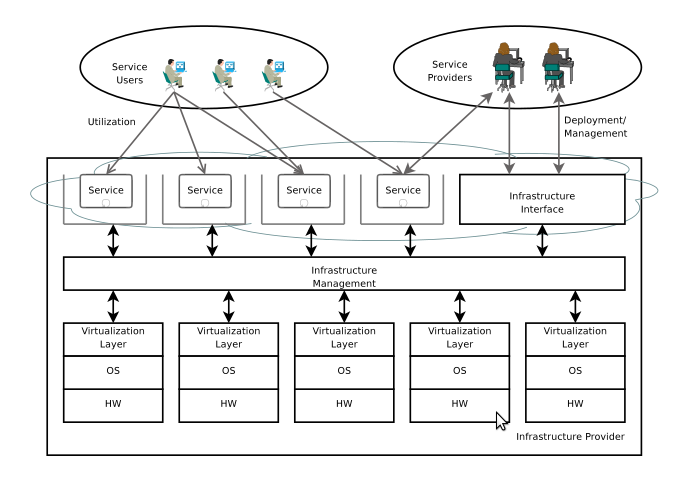
\includegraphics[width=\linewidth]{cloud_actors}
    \caption{Cloud Actors~\cite{Buyya2009599}.}
    \label{fig:cloud_actors}
  \end{center}
\end{figure}

\textbf{The actors:}\\
Service Providers make services accessible to Service Users through Internet-based Interfaces. The computing infrastructure is offered “as a service” by the Infrastructure Providers, moving computing resources from the SPs to the IPs, in order to give the firsts flexibility and reduced costs.

\textbf{The scenarios:}
\begin{itemize}
\item Infrastructure as a Service – IPs are responsible for the management of a large set of computing resources, such as storing and processing capacity. If they use virtualization, they can split, assign and dynamically resize the resources to build ad-hoc systems as the customers (SPs) demand, by deploying the software stacks that run their services.
\item Platform as a Service – Clouds offer an additional abstraction layer – they can provide the software platform where systems run on. The sizing of the hardware resources demanded by the execution of the services is made in a transparent manner. The applications developed are run on the provider's infrastructure and are delivered through the Internet from the provider's servers. The Google Apps Engine is a very good example.
\item Software as a Service – Cloud systems can host many services that users can be interested in, such as online word processors or even Google Apps. \cite{knorr,vaquero}
\end{itemize}

In the article written by Vaquero et al, many Cloud definitions are gathered. Markus Klems states that the key elements for the Cloud are immediate scalability and the optimization of resources usage, these being bring provided by increased monitoring and automation of resources management. Jeff Kaplan and Reuven Cohen prefer to focus on the business model, paying more attention to the collaboration and pay-as-you-go and reducing the costs of investment. Douglas Gourlay and Kirill Sheynkman define the Cloud as being simple virtualized hardware and software, combined with monitoring and provisioning technologies. \cite{21experts,vaquero}

McFedries believes that the basic unit of the Cloud is nothing other than data centers - huge collection of clusters - that can offer a large supply of computing power and storage simply by using whatever resources they can spare.\cite{ieees}

Kevin Hartig defines Cloud Computing as being able to access resources and services needed to perform certain tasks with needs that are constantly changing. The application or user requests access from the cloud rather than on a specific endpoint of the network or a resource. The Cloud becomes a virtualization of resources that is both self maintainable and manageable, a view also shared by Jan Pritzker, who focuses his definition on virtualization and on-demand resource allocation. Other authors such as Reuven Cohen, Praising Gaw, Damon Edwards and Ben Kepes (to name a few) are strong believers that Cloud computing is nothing more other than a buzz word, grouping concepts such as deployment, load balancing, provisioning and data and processing outsourcing.\cite{21experts}

Having this in mind, Vaquero et al believe that the Cloud is a large pool of easily usable and accessible virtualized resources (such as hardware, development platforms and/or services), these being dynamically reconfigured to adjust to a variable load (scaling) also allowing for an optimum resource utilization. The pool of resources is typically exploited by a pay-per-use model in which guarantees are offered by the Infrastructure Provider by means of customized Service-Level Agreements. The authors also state the set of features that resemble this minimum definition would be scalability, pay-per-use utility model and virtualization. \cite{vaquero}

Brian Hayes states in his article that even though the future of Cloud computing is still unclear, there are a few directions in which it can go. One of those directions is Web based services, such as Google Docs or even Photoshop Express. Salesforce.com also offers a variety of online applications and its slogan is actually "No software!". 

As mentioned earlier in the report, Amazon.com also ventured into this new paradigm, offering data storage and computing capacity, each of these services being able to expand and contract as the users need (elasticity) and Google has its App Engine, providing hosting on Google server farms.

There is great concern in terms of scalability in the Cloud, as it might be necessary to organize resources so that the program runs flawlessly even though the number of concurrent users increases might arise. Hayes also mentions that Cloud computing raises questions in terms of privacy, security and reliability, since personal documents are being delivered to a third-party service.\cite{hayes}

Nicholas Carr writes in his book that a shift is happening, where the Cloud is becoming similar (if not equal) to the electric grid, as we can connect to the Cloud and get data, storage space and processing power cheaply and instantly (Utility Computing). \cite{carr}

Aaron Weiss writes in his article that the Cloud is robust, even self-healing, as it has many sources from where to get the power to recover from whatever accident occurs. Weiss states that the Cloud is also very power consuming, as roughly 50 percent of the energy it consumes comes from the cooling process alone. Giants such as IBM and Microsoft are also scouting locations where the hydroelectric power is cheaper and greener, so they can establish their cluster centers.\cite{aaron-clouds}



\subsection{Utility Computing} \label{utility}

Computing is going in such a direction that the services that are made available to the user are being done in such a way that computing is becoming equal to traditional utilities such as water, gas, electricity and telephone services.\cite{Buyya2009599}

In an article published by InfoWorld (formerly the Intelligent Machines Journal), Utility computing is mentioned as being a form of Cloud computing, where storage and virtual servers are being offered and can be accessed on demand, such as the services offered by Amazon.com, Sun or IBM. \cite{grids-and-clouds}

IBM Global Services provide the following definition for Utility Computing:

\begin{quote}
``Utility computing is the on demand delivery of infrastructure, applications, and business processes in a security-rich, shared, scalable, and standards-based computer environment over the Internet for a fee. Customers will tap into IT\footnote{Information Technologies} resources - and pay for them - as easily as they now get their electricity and water.''~\cite{ibm-utility}
\end{quote}

Utilities have the following characteristics:
\begin{itemize}
\item Necessity - Users depend on utility services to fulfill their day-to-day needs. It takes time for distribution networks to spread and costs to decline, as it also takes time for users to adapt to the service. Once they do, the service may grow in importance as users begin to find new ways to reap benefits from it;
\item Reliability - The service must be readily available when and where the user requires it, as a temporal or intermittent loss of service may cause several issues to the user. Redundancy must be built into production capacity in order to make up for hypothetical service failures;
\item Usability - Users have a ``plug-and-play'' mentality and they need to feel at ease with whatever feature they are using;
\item Utilization rates - Utilities are driven by a necessity to carefully manage utilization rates. User demands for utility serves mays vary over time and across service regions. This may lead to spikes in utilization of the service and under-utilization in off-peak periods. Service providers must have in mind that how the service is billed may influence how users use that service;
\item Scalability - As production capacity grows, the unit cost of production shrinks. It might be expected that as the demand for the service rises, the quality of service may decline or vice-versa~\cite{ibm-utility}.
\end{itemize}

Bhattacharya and Vashistha state that utility based computing allows computing resources to be available for a customer on demand, as the customers subscribe to the services of the utility provider and only pay for the quantum of the resources used. This allows any customer to cut down on IT infrastructure spendings as they can simply subscribe to the provider's services and use the computing resources at will, only paying for as much as they use. Typical measures of usage include metered CPU hours and memory space usage~\cite{bhatta-utility}.

Ross and Westerman write in their article that utility computing relies on several important technical capabilities to deliver what it promises - services available on-demand. The authors believe that for most firms, the impact of utility computing will be on the extent and nature of outsourcing. The benefits that can be obtained only enhance the current benefits of IT and business processes outsourcing: lower cost, variable capacity and increased strategic focus. On demand capacity leads to firms to invest less in computing capacity. Advances in autonomic computing may reduce the number of people needed to monitor operations and thus reduce labor costs.

The authors believe that firms will be able to do more with less and will be able to allocate their most strategic resources to their most strategic opportunities~\cite{ross}.

\section{Grids VS. Clouds} \label{sec:gridsvsclouds}

As one knows, Grids and Clouds share a few goals, such as reducing computing costs and increasing flexibility and reliability through the use of third-party operated hardware.

Vaquero et al lay out a very comprehensive list of features and discuss the similarities and differences between them. The list includes resource sharing, heterogeneity, virtualization, security, the offer of high level services such as metadata search, the awareness of architecture, dependencies and platform, software workflow, scalability and self management, standardization, payment model and quality of service. The list is shown in Figure~\ref{fig:grids_vs_clouds} which is in Appendix~\ref{chap:ap1}.

The authors also believe that Grids are meant to be user friendly, virtualized and automatically scalable utilities, something that steps into the Clouds’ path, but they still need to be able to incorporate virtualization techniques in order to obtain some advantages already present in the use of Clouds, like migrability and hardware level scalability.\cite{vaquero}

A few members of the Enabling Grids for E-sciencE (EGEE, now part of the European Grid Infrastructure) performed a comparative analysis on Grids and Clouds, focusing two implementations of both: the EGEE project for Grid and the \textit{Amazon Web Service} (AWS) for Cloud, using metrics such as performance, scale, ease of use, costs and functionality, amongst others. The Grid in use by the EGEE runs on gLite, an open source software which had development funding from the EGEE, described in a later section of this document, as it is used in some extent by FEUP's cluster system.

When comparing both EGEE Grid and the \textit{Amazon Web Service}, the authors of the analysis encounter a set of differences and similarities:
\begin{itemize}
\item The AWS does not expose how they operate their data centers and how they implement the user interfaces, execute the user requests and maintain their accounting, its back-end is still a grey area;
\item The EGEE Grid exposes both user interface as well as the resource interface to permit providers to connect their resources. The AWS hides this second interface;
\item The authors assume that on the resource side, both systems work in similar manner, as both cases require a queueing mechanism whether the data center is dispatching a grid job via a batch system or is requested to instantiate a new virtual machine;
\item The greatest benefit of the Cloud proposed by Amazon is its interfaces and usage patterns, focused on simplicity;
\item Both services are not fail-proof, but the authors consider that a centralized Cloud might not be able to provide the resilience that the distributed nature of EGEE does;
\item Grids are typically used for job execution - limited duration execution of a program, part of a larger set of jobs, consuming or producing a significant amount of data. Clouds, even though they support a job usage pattern, they seem to be more often used for long-serving services;
\item Amazon bills users for computing resources usage with a minimum of one hour usage. This stops being efficient when dealing with a large number of small jobs;
\item Elasticity in the Grid is made by adding worker nodes at a site or adding new sites;
\item The complexity in the Cloud is kept server-side, which makes its entry point very low, something that is still considered a goal to achieve for Grids. \cite{grids-and-clouds}
\end{itemize}


\section{Developments, Applications and Services}
With the shift of the computing industry towards a provision of Platform as Service and Software as a Service, consumers can access resources on-demand without having to preoccupy themselves with time and location, Buyya et al believe that there will be an increasing number of Cloud platforms being developed.~\cite{Buyya2009599} One of those platforms is \textit{OpenNebula}, an open-source tool kit for Cloud management. In this report, the Amazon computing service (\ref{aws}) will also be analysed, as well as \textit{Google's App Engine} (\ref{googleapps}) and \textit{Microsoft Azure} (\ref{azure}).
\textit{Rackspace Hosting} and \textit{NASA}'s \textit{OpenStack} 

\subsection{AWS - Amazon Web Services}\label{aws}

The \textit{Amazon Web Services} consist of several components, but only two will be taken into consideration in this document, as they are the most relevant to the work discussed: \textit{Amazon's Simple Storage System} (\ref{amazon-sss}) and \textit{Amazon's Elastic Computing Cloud} (\ref{amazon-ec}).

\subsubsection{Amazon's Simple Storage Service}\label{amazon-sss}

The core service for the \textit{Amazon Web Services} is the \textit{Amazon's Simple Storage Service}, that gives the user the power to store large amounts of data in a reliable way which does not hinder its availability. Data is accessed through protocols such as SOAP\footnote{Simple Object Access Protocol - Used to exchange information in the implementation of Web Services in computer networks.} and REST\footnote{Representational State Transfer - Style of software architecture for distributed hypermedia such as the World Wide Web.}, while also being able to be accessible via normal web browsers.
The storage model runs on a two-level hierarchy, where the users can create \textit{buckets} and place data \textit{objects} in those buckets. Strings are used as keys for both buckets and objects, thus being able to be easily incorporated in URLs. Users are charged 15 US cents per Gigabyte per month, each user being able to have up to 100 buckets and each can hold up to 5GB of data.\cite{hazel}

\subsubsection{Amazon's Elastic Computing Cloud}\label{amazon-ec}

Physically speaking, the \textit{Elastic Computing Cloud} (EC2) is a large number of computers on which Amazon provides time to paying customers, these computers being spread all over the United States. EC2 is based on the XEN virtualization technology, which allows one physical computer to be shared by several virtual ones, each with its own operating system.

Through the use of virtualization, the users create an image of their software environment using the tools provided. This will be used to create and instance of a machine in Amazon's Cloud. Customers can freely choose configuration templates for their instance and they can create and destroy the instances at will, enabling the software to scale itself to the amount of computing power it needs.\cite{grids-and-clouds, hazel}

Amazon has released \textit{Elastic IPs} (Static IPs for Dynamic Cloud Computing), which allows the assignment of static IPs to dynamic resources that are deployed via EC2, as well a service that enables users to request EC2 instances to be geographically distributed, as a response to the demand for EC2 IP addresses in a static range for application range for applications like email service hosting, as well as providing a safety net in case the operations of an Amazon Web Services data center go awry. 

Amazon provides a variety of ways of requesting the EC2 instances, namely through the use of Web Services, supporting Buyya et al's Cloud definition previously mentioned in the document.

Amazon has also introduced its own performance unit named "EC2 Compute Unit". Since Amazon ventured into the Utility computing field, model it follows differs from the traditional way developers were formatted to think about CPU resources. Instead of renting a certain processor for several months or years, it is now rented by the hour. One EC2 Compute Unit provides the CPU equivalent of a 1.0-1.2 GHz 2007 Opteron or 2007 Xeon processor.\cite{amazon-aws}

\subsection{Google Cloud - Google's App Engine}\label{googleapps}

The \textit{Google Cloud}'s official name is \textit{App Engine} or \textit{Appengine}. It gives developers the ability to run web applications on Google's infrastructure, the same that is being used by \textit{Google} for \textit{GMail} and \textit{Google Docs}.
The Cloud appears to be a platform accessible over the Internet with limitless hardware, the latest software and abundant storage for deploying web applications.
The \textit{App Engine} has the following features:
\begin{itemize}
\item Automatic horizontal scaling and load balancing;
\item APIs\footnote{Application Programming Interface} for authenticating users with Google Accounts and for sending emails. No system administration is needed by the user to set up or allow access to these APIs;
\item Fully featured Eclipse developed environment that simulates \textit{Google App Engine} on the localhost for development and testing;
\item Persistent storage and support for transactions and queries using the standard JDO\footnote{Java Data Objects} and JPA\footnote{Java Persistence API} APIs;
\item Generous free quotas, which allow small universities to have access to the same hardware and software as large industries. Each user can have 10 applications created, each with 10 versions, which totals an effective development environment of 100 applications. A free account supports six and a half CPU hours a day, with 1GB of stored data and sending email to 2000 recipients a day and a max of 5 million page views a month;
\item It is free, with no contracts to sign, no hardware expense and no system administration costs for maintaining, updating, patching or backing up \textit{App Engine};
\item Eclipse plug-in available for Apple, Linux and Windows, which allows standard debugging using Eclipse debug tools. It provides menu based functionality to automatically upload the application to the Google App Engine;
\item Requires no system administration;
\item Simple web based, user friendly console.\cite{googleapp}
\end{itemize} 

\subsection{Microsoft Azure}\label{azure}

\textit{Microsoft Azure} platform is a cloud computing platform which offers a set of cloud computing services similar to those offered by Amazon Web Services. \textit{Windows Azure Compute} (Microsoft's counterpart to Amazon's EC2), only supports Windows virtual machines and offers a limited variety of instance types when compared with Amazon's EC2. Its instance type configurations and cost scales up linearly from small to extra large and its instances are available in 64 bit x86\_64 environments. 

It has been speculated that the clock speed of a single CPU core in \textit{Azure}'s terminology is approximately 1.5 GHz to 1.7 GHz.\cite{azure-paper}
Windows Azure enables developers to build, host and scale applications in Microsoft datacenters, not requiring upfront expenses, long term commitment and users only pay for the resources they use. 
Windows Azure relieves the user from the effort of configuring load balancing and failover, is designed to let developers build applications that are continuously available, even if they need software updates and hardware failures occur.\cite{azure}

\clearpage
\section{FEUP's Computing System}\label{feup}

In this section FEUP's computing system is analyzed in detail. The cluster system and the technologies it uses in its management are described and detailed. FEUP's cluster system currently uses three different technologies, \textit{Moab}, \textit{gLite} and \textit{Condor}.
The Cloud creation and management tool is also described, as it is a vital part in FEUP's computing system and is the connecting link between the front-end and the back-end.

\subsection{OpenNebula}\label{subsec:opennebula}


\textit{OpenNebula} was initially created as a research project in 2005 by Ignacio M. Llorente and Rubén S. Montero from \textit{Universidad Complutense Madrid}, being publicly released in 2008. It now works as an open source project after having evolved through several releases (now on version 3.4). It is the result of many years of research and development in efficient and scalable management of virtual machines on large-scale distributed infrastructures in close collaboration with \textit{OpenNebula}'s user community and leading experts in cloud computing. 

Most of \textit{OpenNebula}'s features have been developed as a response to the use cases from many of the companies involved in the project (these include RESERVOIR~\footnote{\textit{Framework} developed to aid both techonology and information specialists in enterprises in creating a cloud with all the coding and architecture specifications needed.~\cite{http://www.reservoir-fp7.eu/}}, \textit{StratusLab}~\footnote{A project aiming to develop a complete and open-source cloud distribution that allows both grid and non-grid resource centers to offer and exploit an IaaS cloud. It is particularly focused on enhancing distributed computing infrastructures such as the European Grid Infrastructure (EGI)~\cite{startuslab.eu}} and \textit{4CaaSt}~\footnote{Project created for the development of an advanced PaaS cloud platform which supports the optimized and elastic hosting of Internet-scale multitier applications, embedding all the necessary features, so that the programming of rich applications is simplified.~\cite{http://4caast.morfeo-project.org/}}) and its technology has evolved mostly thanks to the effort the community has.~\cite{opennebula_site}

It was first released as a software package in \textit{Ubuntu} 9.04, has its own command-line tools and gives the user different configuration scripts which enable a simple and flexible way to design and manage running virtual machines. Since the release of version 3.0, \textit{OpenNebula} has introduced a GUI called \textit{Sunstone} (only runs on \textit{Firefox} and \textit{Chrome} browsers), which allow the users and administrators to manage all \textit{OpenNebula}'s resources (as long as they have access to them, something that can be regulated via ACLs or external modules)~\cite{jorge-ruao}.

\textit{OpenNebula}'s architecture is presented in Figure~\ref{fig:nebula_arch} and its main components are presented in Figure~\ref{fig:nebula_components}.

\begin{figure}[h!]
  \begin{center}
    \leavevmode
    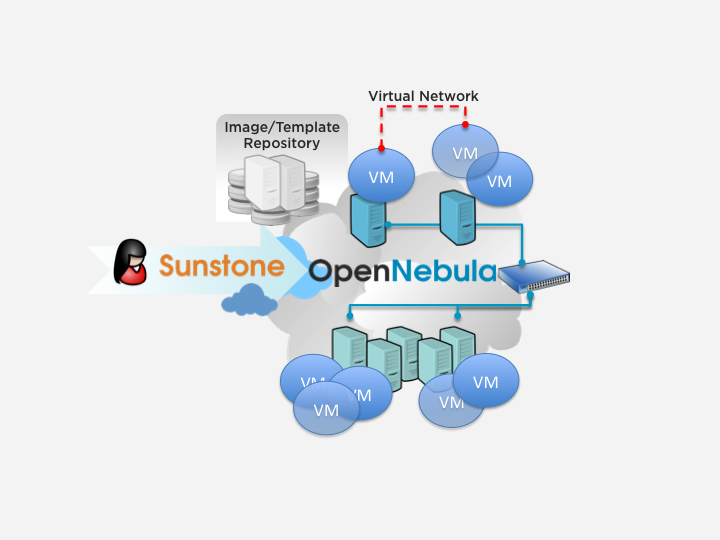
\includegraphics[scale=0.5]{nebula_arch}
    \caption{OpenNebula's Architecture~\cite{http://opennebula.org/about:technology}.}
    \label{fig:nebula_arch}
  \end{center}
\end{figure}

\begin{figure}[h!]
  \begin{center}
    \leavevmode
    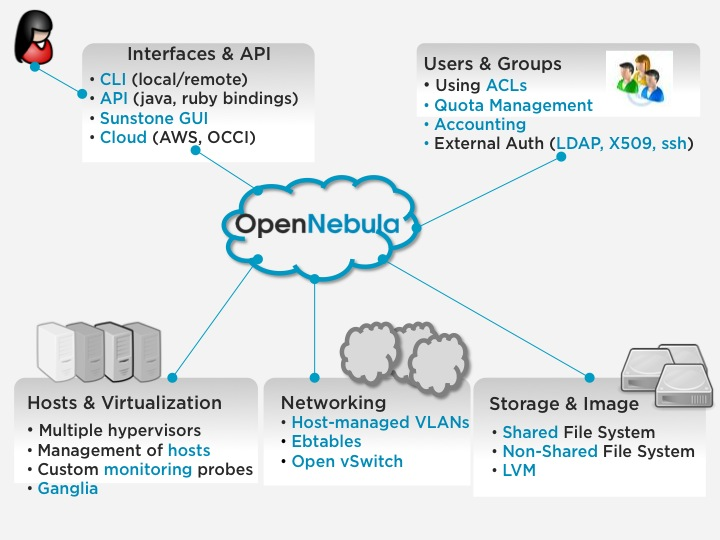
\includegraphics[scale=0.5]{nebula_components}
    \caption{OpenNebula's components~\cite{http://www.opennebula.org/documentation:rel3.4}.}
    \label{fig:nebula_components}
  \end{center} 
\end{figure}


\begin{itemize}
\item \textbf{Interfaces and APIs} --- \textit{OpenNebula} offers two main ways to manage its instances: CLI or GUI (\textit{Sunstone}). Several cloud interfaces such as \textit{OCCI}~\footnote{Open Cloud Computing Interface. Web service that enables the user to launch and manage virtual machines in the \textit{OpenNebula} installation.} and EC2 Query~\footnote{Web service that enables the use of virtual machines through Amazon's EC2 Query Interface (\ref{amazon-ec})};
\item \textbf{Users and Groups} --- \textit{OpenNebula} supports user accounts and groups, as well as several authentication and authorization mechanisms. These can be used to create isolated compartments inside the same cloud (multi-tenancy). An ACL mechanist also exists to allow different role management;
\item \textbf{Hosts} --- Various hypervisors are supported by the virtualization manager, which has the ability to control and monitor the lifecycle of VMs, something that can be extended to the physical hosts. It is compatible with Xen, KVM and VMware, three \textit{platform virtual machines} that emulate the whole physical computer machine;
\item \textbf{Networking} --- A network subsystem that allows \textit{OpenNebula} to easily integrate with specific network requirements of existing datacenters;
\item \textbf{Storage} --- \textit{OpenNebula} supports multiple data stores in its storage subsystem which provides extreme flexibility in planning the storage backend. Disk images can be stored in both file and block device, also having support for the VMware datastore;
\item \textbf{Clusters} --- Clusters are pools of hosts that share datastores and virtual networks. They are used for load balancing, high availability and high performance computing.
\end{itemize}
\textit{OpenNebula} does not have a built-in utility to create VMs from scratch, but its templates allow the VMs to boot an ISO image, leaving the user with just creating an empty hard disk image.

It provides monitoring capabilities which become rather useful when there is a need to troubleshoot, scale or control resource allocation scenarios. \textit{OpenNebula} exports drivers that communicate directly with the hypervisor (KVM - \ref{hyper}) and return useful data, such as the amount of CPU used, reserved and used memory and network traffic.\cite{open-clouds}

In March 2010, \textit{OpenNebula}'s main authors founded \textit{C12G Labs}~\footnote{Company that provides enterprise-grade solutions built around \textit{OpenNebula}}, which has led to it being referred to as "...proprietary tech with an element of openness...", which could limit its growth.~\cite{http://www.linkedin.com/groups/OpenStack-vs-Eucalyptus-vs-OpenNebula-2685473.S.54382975}

%\clearpage
\subsection{OpenStack}\label{subsec:openstack}

\textit{OpenStack} is a global collaboration of developers and cloud computing technologists producing the open source cloud computing platform for public and private clouds. The aim of this project is to deliver solutions for all types of clouds by being simple to implement, massively scalable and filled with features. 

First released in October 2010 and now on its fifth version (codename Essex), OpenStack has undergone major changes and revamps over the past months ~\cite{openstack}.

It was founded by \textit{Rackspace Hosting} and NASA\footnote{North American Space Agency} (deployed as NASA's Nebula cloud\cite{needs cite})and it has grown to be a global software community of developers collaborating on a standard open source cloud operating system. Current \textit{OpenStack} ``controllers'' include \textit{OpenStack Foundation}, \textit{Canonical}, \textit{Cisco}, \textit{Dell}, \textit{Red Hat}, \textit{SUSE} and \textit{Yahoo!}. \cite{https://github.com/dellcloudedge/crowbar/wiki/OpenStack-Essex-Deploy-Day}

\textit{OpenStack}'s mission is to enable any organization to create and offer cloud computing services running on standard hardware.

All of its code is available under the \textit{Apache} 2.0 license and as such, anyone can run it, build applications on it or submit changes back to the project. It is commoditizing the IaaS market, enabling the users to get from \textit{Amazon} today into their own private data centers and cloud environments by using open source. \cite{https://github.com/dellcloudedge/crowbar/wiki/OpenStack-Essex-Deploy-Day}

\subsubsection{OpenStack Architecture}\label{subsubsec:openstack_arch}
  
The following figure depicts OpenStack's software diagram:

\begin{figure}[h]
  \begin{center}
    \leavevmode
    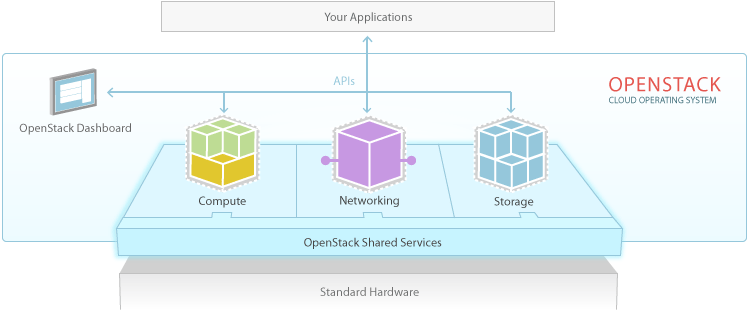
\includegraphics[width=\textwidth]{openstack-software-diagram}
    \caption{OpenStack Software Diagram\cite{openstack}.}
    \label{fig:openstack_sw_diag}
  \end{center}
\end{figure}

\textit{OpenStack} has four major components:

\begin{itemize}
\item \textbf{Compute} - Also known as \textit{Nova}, it is designed to provision and manage large networks of virtual machines. Provides an API so that developers who wish to build cloud applications can access the compute resources, as well as web interfaces for administrators and users. Its architecture is designed to be flexible in the cloud design, so that no proprietary hardware or software is required and has the ability to integrate with legacy systems and third party technologies. \textit{Nova} can manage and automate pools of compute resources and works with a great deal of virtualization technologies, enabling the administrators to use multiple hypervisors, such as KVM or XenServer.
\item \textbf{Networking} - A pluggable, scalable and API-driven system for managing networks and IP addresses. Keeps the network from bottlenecking or being a limitation factor in the cloud deployment. Designed to provide flexible networking models to cater the needs of different applications and user groups. Manages IP addresses, allowing both static IPs or DHCP. Allows the administrator or the user to reroute traffic in case of maintenance or failure. \textit{OpenStack Networking} has an extension framework which allows extra network services, such as intrusion detection systems, firewalls and VPNs to be deployed and managed.
\item \textbf{Storage} - Also known as \textit{Swift}, it is ideal for cost effective and scale-out storage~\footnote{A storage system that uses a scaling methodology in order to create a dynamic storage environment which will support balanced data growth on an as-needed basis. Its architecture uses a number of storage nods that are configured to create a storage pool or are configured to increase computing power and is designed to scale boyth capacity and performance~\cite{http://www.webopedia.com/TERM/S/scale_out_storage.html}}. It has a fully distributed and API-accessible storage platform which can be integrated directly into applications or used as a backup, achiving and data retention tool. It allows for block devices to be exposed and connected to compute instances for expanded storage, better performance and integration with enterprise storage platforms. \textit{OpenStack Swift}'s object storage is a distributed storage system for static data such as VM images, photo and email storage, backups and archives. It has no central point of control thus providing greater scalability, redunndancy and durability. Storage clusters can scale horizontally by adding new servers. If one of the servers or a hard drive fails, OpenStack replicates its content from other active nodes to a new location in the cluster. Furthermore, \textit{OpenStack} uses algorithms in order to replicate and distribute data accross different devices which allows for the use of inexpensive hard drives and servers.
\item \textbf{OpenStack Dashboard} - Also known as \textit{Horizon}, it provides administrators and users with a GUI to access, provision and automate cloud-based resources. It is extensible, making it easy to attach third party services, such as billing, monitoring and additional management tools. It is a simpler way to access the resources, which can also be done by building their own tools using either \textit{OpenStack}'s or EC2' compatible API.
\end{itemize}

Alongside the four components described above, \textit{OpenStack} also has a few shared services which make implementing and controlling the cloud an easier job. They are designed in a way that they can integrate with themselves as well as the components above.

\textit{OpenStack} has its own identity service - named \textit{Keystone} - which shows a central directory of users mapped to the \textit{OpenStack} services they can access. \textit{Keystone} acts as a common authentication system accross the operating system that the cloud sits on and can integrate with existing backend services such as LDAP. This identity service allows the administrator to configure centralized policies accross the users and systems as well as defining permissions for the four major components depicted above, whereas the users can get a list of services they can access, make API requests or log into the web dashboard - \textit{Horizon} - to create resources linked to their account.

Another important serviced provided by \textit{OpenStack} is its image service \textit{Glance}. It provides discovery, registration and delivery services for disk and server images. It has the ability to snapshot a server image and store it, which can then be used as a template to get new servers up and running very quickly - and consitently in the case of setting up multiple servers - rather than installing a server OS and individually configuring the additional services required. \textit{Glance} can store both disk and server images in a great variety of backends, including \textit{OpenStack}'s own object storage. A standard REST interface is provided for querying information on disk images and that lets clients stream the images to new servers. The image registry supports a wide range of formats, which include images generated by KVM, Qemu, VMWARE and RAW images.

This project is under close surveillance by CICA as it is viewed as a possible substitute for \textit{OpenNebula} (\ref{opennebula}). \textit{OpenStack} is also discussed in the following chapter~\ref{chap:chap3} as it is one of the focuses of the work realized.

\subsubsection{DevStack}\label{subsubsec:devstack}

Since \textit{OpenStack} still has a somewhat complex deployment process, \textit{DevStack} was created in order to provide whoever wishes to try out \textit{OpenStack} for development purposes.

It is essentially a set of scripts and utilities to quickly deploy an \textit{OpenStack} cloud.

Its goals include the following:
\begin{itemize}
\item To enable the user to quickly build dev \textit{OpenStack} environments in a clean Ubuntu or Fedora environment;
\item To describe working configurations of \textit{OpenStack};
\item To make it easier for developers to get familiar with \textit{OpenStack} without the need to understand every single part of the system at once.
\end{itemize}


Created by \textit{Rackspace Cloud Builders}~\footnote{Business launched by \textit{Rackspace} that helps other businesses deploy \textit{OpenStack}~\cite{http://www.rackspace.com/cloud/private_edition/}}, \textit{DevStack} will be used as it simplifies the deployment process (and is used by FEUP's \textit{OpenStack} researcher). \textit{DevStack} will be further expanded in Chapter~\ref{chap:chap3}, when its deployment is discussed.

\subsection{Clusters}\label{clusters}

Three different technologies are currently in use by FEUP's Cluster system: \textit{Moab}(\ref{moab}), \textit{gLite}(\ref{glite}) and \textit{Condor}(\ref{condor}).

\subsubsection{Moab Cluster Suite}\label{moab}

\textit{Moab Cluster Suite} is a proprietary tool for high performance computing systems, developed by the company \textit{Cluster Resources}. It has built-in modules for work management, Cluster administration and monitoring, report creation. It is composed by three essential components:
\begin{itemize}
\item \textbf{Moab Workload Manager} - scheduling and workload management engine;
\item \textbf{Moab Cluster Manager} - graphical interface for Cluster administration, monitoring and report analysis;
\item \textbf{Moab Access Portal} - web based portal for job management and submission, directly focused on the end-user.
\end{itemize}

A resource manager supplies the system with basic functionalities for initiating, stopping, canceling or monitoring jobs. \textit{Moab Workload Manager} uses a resource manager's services to get information about the state of the resources and the node workload. It is also used to manage jobs and to send information on how they should be run and it can be configured to manage more than one resource manager simultaneously.
Its composing nodes can be split into three groups:
\begin{enumerate}
\item \textbf{Master node} - Manages the resources;
\item \textbf{Submissive/Interactive nodes} - Allow users to manage and submit jobs into the system;
\item \textbf{Computing nodes} - Execute the submitted jobs.
\end{enumerate}

Is is also possible to split the nodes into two groups - source and destination nodes. The first ones are the nodes where there users, portals or other systems can submit their jobs and the latter ones are where the jobs are executed. Jobs originate in a source node and are transferred to the destination nodes. Decisions are made in the source nodes, so it is possible to choose which nodes will execute the submitted jobs.
Moab also allows for the establishment of connections between several Grid systems, which permit access to additional resources.\cite{jorge-ruao, moab}


\subsubsection{gLite}\label{glite}

\textit{gLite} consists in a set of components designed with the objective of building a Grid computing infrastructure for resource sharing developed by the project EGEE (Enabling Grids for E-sciencE), also mentioned in an earlier section.
\textit{gLite} is based on four core concepts:
\begin{itemize}
\item \textbf{Computing Element (CE)} - Set of local computational resources, namely a Cluster. It is composed by three components:
	\begin{itemize}
	\item \textbf{Grid Gate} - generic interface for the Cluster who receives jobs and submits it to the Local Resource Management System (LRMS);
	\item \textbf{Local Resource Management System (LRMS)} - Sends the jobs to the worker nodes for execution;
	\item \textbf{Worker Nodes} - Cluster nodes where jobs are executed.
	\end{itemize}
\item \textbf{Storage Element (SE)} - Supplies access to data storage resources;
\item \textbf{Information Service (IS)} - Resource research is made through this component, which is also responsible for supplying information regarding resources and their state;
\item \textbf{Workload Management System (WMS)} - Receives jobs from users, appropriately allocates a CE, saves jobs states and gets the final results.\cite{jorge-ruao,glite}
\end{itemize}

\subsubsection{Condor}\label{condor}

\textit{Condor} is a free and open-source workload management system, developed by the \textit{Condor Research Project}.
It has built-in job queueing mechanisms, scheduling and priority policies, resource monitoring and management. Users submit jobs to \textit{Condor}, which puts them in a queue, chooses when and where to execute them based on defined policies, carefully monitors their progress and informs the user when the jobs are finished.
\textit{Condor} can manage dedicated nodes or harness the CPU energy wasted in workstations that are turned on but unused. If the system detects the machine became suddenly unavailable, \textit{Condor} can migrate the state of the job into a different machine and resume work. 
It offers an extremely flexible structure to assign resources to jobs, allowing these to have specific requisites and resource preferences, as well as enabling the resources to specify preferences over jobs to execute.
Each machine from \textit{Condor} can play several roles:
\begin{itemize}
\item Central Manager - Machine that collects information and makes the negotiation between resources and resource requests. All resource requests go through the \textit{Central Manager}. There can only be one \textit{Central Manager} in a \textit{Condor} infrastructure;
\item Execute - Machine which executes jobs, therefore allowing the network to take advantage of its resources. Any machine can be configured to take this role;
\item Submit - Machine responsible for the job reception and submission to the \textit{Central Manager}. Any machine can be configured to take this role;
\item Checkpoint Server - Machine which stores checkpoint files for all submitted jobs.\cite{jorge-ruao,condor}
\end{itemize}


\section{ISO Images} \label{iso}

unsure.....

Ubuntu's VM Builder? talvez ver mais.


\section*{}

Neste capítulo é descrito o estado da arte e são
apresentados trabalhos relacionados para mostrar o que existe no
mesmo domínio e quais os problemas em aberto.
Deve deixar claro que existe uma oportunidade de desenvolvimento que
cobre alguma falha concreta .

O capítulo deve também efectuar uma revisão tecnológica às principais
ferramentas utilizáveis no âmbito do projecto, justificando futuras
escolhas.


\section{Resumo ou Conclusões}

No final do capítulo deverá ser apresentado um resumo com as 
principais conclusões que se podem tirar. 

Vivamus non nunc nec risus tempor varius. Quisque bibendum mi at
dolor. Aliquam consectetuer condimentum risus. Aliquam luctus pulvinar
sem. Duis aliquam, urna et vulputate tristique, dui elit aliquet nibh,
vel dignissim magna turpis id sapien. Duis commodo sem id
quam. Phasellus dolor. Class aptent taciti sociosqu ad litora torquent
per conubia nostra, per inceptos himenaeos. 

\chapter{Problem Statement} \label{chap:chap3}

In this chapter the problem will be described and justified, using references from the bibliographic study presented in Chapter~\ref{chap:sota}.

\section{Problem Description}

Currently, FEUP's computing infrastructures are only accessed by those who have the technical knowledge to interact with the system. These people are technicians whose area of expertise encompasses outsourcing computing resources to perform computing jobs. 

If someone from an area unrelated to the computing system wants to perform any operation in it, that someone must contact the said technicians and waste valuable time for both parties cutting through red tape.

Having this in mind, CICA has started developing a project that reduces the amount of knowledge necessary to perform the said computing operations.

This document focuses only on the front-end of the project, the back-end having already been developed by former MIEIC student Nuno Cardoso as part of his Master Thesis. CICA's project is described in greater detail in the following section.

\section{The project} \label{sec:project}


The project aims at simplifying the whole process and to make FEUP's computing infrastructures more accessible to the academic community, without the users having to spend time learning about the technologies and how the system actually works.

In order to better understand the full scope of the issue, Figure~\ref{fig:big_picture} shows the full system as it should function, through the means of an hypotetic and yet plausible use case scenario:

\begin{figure}[h!]
  \begin{center}
    \leavevmode
    \fbox{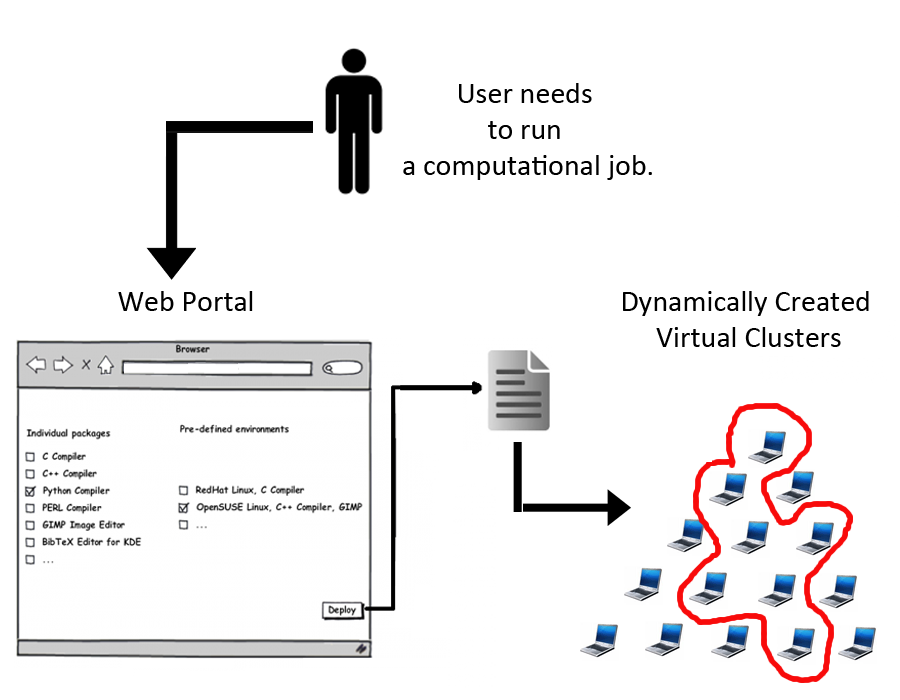
\includegraphics[width=\linewidth]{big_picture.png}}
    \caption{CICA's full computing project.}
    \label{fig:big_picture}
  \end{center}
\end{figure}

Firstly, a researcher of a specific field of study wants to conduct a more complex operation that involves greater computing efforts than his/her home and work computer. As such, the researcher proceeds to enter the designed system through a web page where he/she can:

\begin{itemize}
	\item Chose a suitable work environment for his/her computational needs according to a set of predefined parameters;
	\item Create his/her own work environment according to the specifications he/she provides the system with.
\end{itemize}

The system will then automatically create a virtual environment (image containing all the information needed), which will be passed onto the back-end of the project where a virtual cluster will be created according to that virtual environment.
Finally a username and password combination should be returned so that the researcher can enter the created environment and perform his/her operations. 

The objectives for this project can be divided as following:

\begin{enumerate}
\item Implementing the creation of virtual images;
\item Making the creation according to what the users specify --- image contextualization;
\item Passing the images created to \textit{OpenStack}. This includes connecting with both \textit{Horizon}(dashboard) and \textit{Glance} (image service).
\item Creating a web system that makes the objectives above transparent for the user.
\end{enumerate}


\section{The solution}\label{sec:solution}

As mentioned in the above section, one of the main objectives of this dissertation is the integration of an \textit{OpenStack} --- presented in Chapter~\ref{chap:sota} --- deployment environment as it should simplify the cloud creation and management. 

In this section of this chapter the technological choices are presented and justified.

\subsection{The chosen technologies}\label{subsec:tech}

One thing was missing in the cloud computing scene... A cloud management layer. A cloud operating system that added automation and control at scale. That is where \textit{OpenStack} comes into play. As mentioned in Chapter~\ref{chap:sota}, section~\ref{subsec:openstack} it is built by a world wide community of developers, something that made it a good choice to investigate, as the open source culture is something always worthy of enriching.~\cite{stackgithub}

There is one thing one must keep in mind: as it was described in Chapter~\ref{chap:sota}, \textit{OpenStack} is not the only solution available. \textit{OpenNebula} was also available and is already up and running at FEUP. So why choose \textit{OpenStack}?

First of all, \textit{OpenStack} is a more recent project and \textit{OpenNebula}. It is backed up by some renowned names in the industry, such as \textit{Dell}, \textit{AMD}, \textit{Intel}, \textit{Canonical}, \textit{Cisco}, \textit{StackOps}, \textit{HP}, \textit{NEC}, \textit{AT \& T}, \textit{Yahoo!} and \textit{Red Hat}. Some of these companies also support \textit{OpenNebula}.

The coding activity on both projects was also taken into account when chosing which to deploy. With the help of OHLOH~\footnote{An open source directory that anyone can edit. It features comprehensive metrics and analysis on thousands of open source projects.~\cite{ohloh}}, the differences can be easily observed as it is shown in Figure~\ref{fig:ohloh_compare}, which is included in Appendix~~\ref{chap:ap2}.

\textit{OpenStack} has more favourable statistics, such as the number of committers and number of commits (shown in Figures~\ref{fig:committers} and~\ref{fig:commits}) over time. If this is viewed with the knowledge that \textit{OpenNebula} was created first, and \textit{OpenStack} managed to outdo it, great things can be expected.

\begin{figure}[h]
  \begin{center} 
    \leavevmode 
    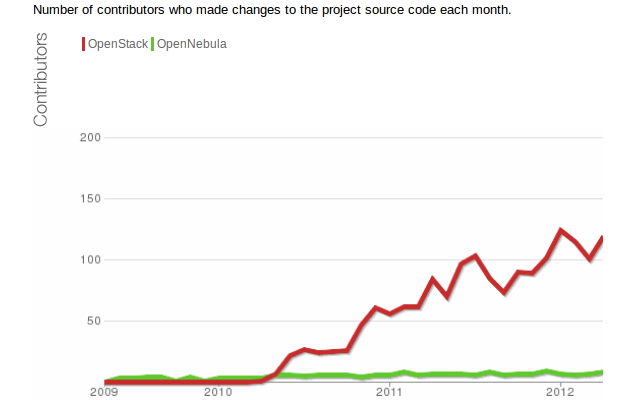
\includegraphics[scale=0.65]{committers}
    \caption{Comparison between the number of committers on \textit{OpenStack} and \textit{OpenNebula}.~\cite{ohloh}} 
    \label{fig:committers} 
  \end{center}
\end{figure}

\begin{figure}[h]
  \begin{center}
    \leavevmode
    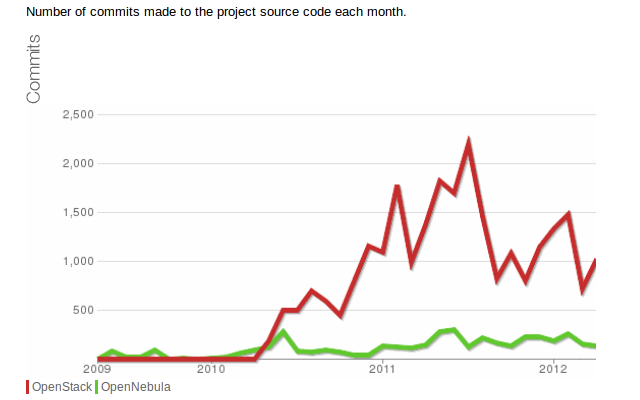
\includegraphics[width=\textwidth]{commits}
    \caption{Comparison between the number of commits on \textit{OpenStack} and \textit{OpenNebula}.~\cite{ohloh}}
    \label{fig:commits}
  \end{center}
\end{figure}

In addition to this and as it was refered in Chapter~\ref{chap:sota}, section~\ref{subsec:opennebula}, \textit{OpenNebula}'s creators have founded an enterprise of their own (C12G Labs) which offers an enterpreise version of \textit{OpenNebula} (named \textit{OpenNebulaPro}). This deviates from the open source philosophy, something that \textit{OpenStack} maintains.

On a more technical aspect, \textit{OpenStack} is mainly written in \textit{Python} whereas \textit{OpenNebula} is mainly coded in \textit{C++} and \textit{Ruby}, as it can be observed in Figure~\ref{fig:code-stack-nebula}. 

In order to understand the relevance of this detail, it must be said that there is an extensive and obligatory contact with \textit{C++} in MIEIC, something that does not happen with \textit{Ruby}, and \textit{Python} is not presented at all. Previous experience with both \textit{C++} and \textit{Ruby} proved to be unfulfilling (\textit{C++} due to its not-so-high-level nature and \textit{Ruby} because it was used in the context of \textit{Ruby on Rails}, which due to some installation quirks was deemed impossible to start and use). 

\textit{Python} on the other hand, was a different programming language, something that was going to be a challenge. Coupled with \textit{Django}, it promised the same advantages as \textit{Ruby on Rails}, but with less trouble getting it up and running. Since \textit{Horizon} is built on \textit{Django}, the choice seemed obvious. The cherry on top of the cake would be contributing to FEUP's knowledge on the new technologies to be researched (\textit{Django}, \textit{Python} and of course, \textit{OpenStack}).

The previous experience with \textit{Ruby} paired with the desire for new challenges and learning new programming languages, \textit{OpenStack} was chosen. This would also allow to contribute to FEUP's knowledge on this new technology.

\begin{figure}[h!]
  \begin{center}
    \leavevmode
    \fbox{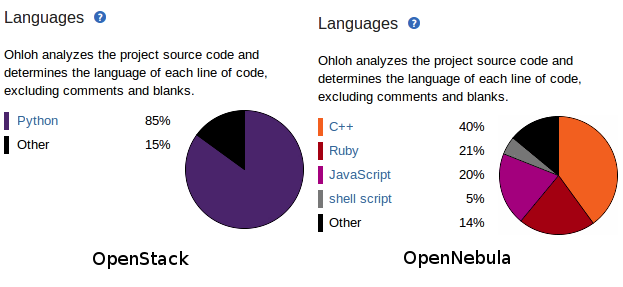
\includegraphics[scale=0.5]{code-stack-nebula}}
    \caption{Comparison between the programming languages in \textit{OpenStack} and \textit{OpenNebula}.~\cite{ohloh}}
    \label{fig:code-stack-nebula}
  \end{center}
\end{figure}

Rodrigo Benzaquen, director of site operations and infrastructure at MercadoLibre, a Latin America e-commerce market leader which chose to use \textit{OpenStack} as their cloud solution, stated the following:

\begin{quote}
 ``Before this [\textit{OpenStack}'s deployment], we would have had someone physically deploy the server which would take a day or longer. With \textit{OpenStack}, we don't have to do that; our developers are now able to create and manage their servers.''\cite{openstack-userstories}
\end{quote}

which came directly into the objective of this dissertation, easing the cloud creation and management process.

\clearpage
\subsection{Connecting the dots}\label{subsec:architecture}

As mentioned in Chapter~\ref{chap:sota}, section~\ref{subsec:openstack}, \textit{OpenStack} is designed to deliver a massively scalable cloud operating system, each of the components being designed to work together in order to prodive complete IaaS. This integration is facilitated through pulic APIs that each service offers, being available to the cloud's end users.~\cite{ken-pepple:essex-arch}. 

Expanding the diagram shown in Figure~\ref{fig:openstack_sw_diag}, the relationships between the services are shown in Figure~\ref{fig:openstack_services}:

\begin{figure}[h!]
  \begin{center}
    \leavevmode
    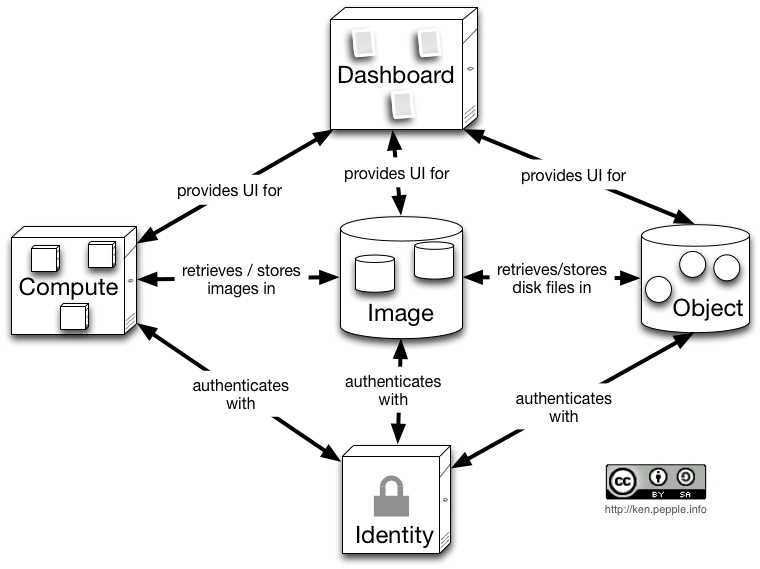
\includegraphics[scale=0.5]{nova-concept-int-essex}
    \caption{Relationships between the different \textit{OpenStack} services.~\cite{ken-pepple:essex-arch}}
    \label{fig:openstack_services}
  \end{center}
\end{figure}

The solution proposed for this project links the \textit{OpenStack} Dashboard --- \textit{Horizon} --- with the designed \textit{Web application} developed in \textit{Python} and \textit{Django}, as shown in Figure~\ref{fig:architecture}.

\begin{figure}[t]
  \begin{center}
    \leavevmode
    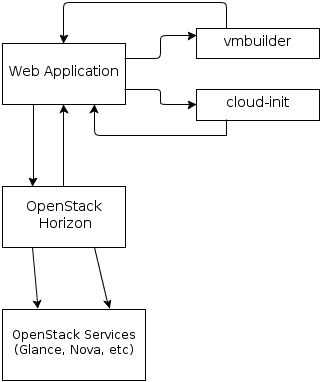
\includegraphics[scale=0.5]{architecture}
    \caption{Proposed architecture implementation.}
    \label{fig:architecture}
  \end{center}
\end{figure}

As it can be observed, the web application will use \texttt{vmbuilder} and \textit{cloudinit} whenever needed and then passing that information to the \textit{OpenStack Horizon} dashboard, which will communicate with the rest of \textit{OpenStack} services.

Since \texttt{vmbuilder} and \textit{cloudinit} work for different purposes (\texttt{vmbuilder} creates contextualized VM images and \textit{cloudinit} contextualizes clean VM images), different tools will be used for different purposes.



An interesting feature to complete in future work could be eliminating the web system and passing the image creation and contextualization to \textit{OpenStack}, modifying the \textit{Horizon} dashboard itself.
 

%Este capítulo deve começar por fazer uma apresentação detalhada do
%problema a resolver\footnote{Na introdução a apresentação do
%  problema foi breve.} podendo mesmo, caso se justifique,
%constituir-se um capítulo com essa finalidade.

%Deve depois dedicar-se à apresentação da solução sem detalhes de
%implementação. 
%Dependendo do trabalho, pode ser uma descrição mais teórica, mais
%``arquitectural'', etc.
%\clearpage
\section{Conclusions}

In this chapter was presented the architecture to be followed in Chapter~\ref{chap:chap4} in the implementation phase of the project. The objectives were also outlined, as well as which technologies to use.

\chapter{Implementação}\label{chap:chap4}

\section*{}

Este capítulo pode ser dedicado à apresentação de detalhes de nível
mais baixo relacionados com o enquadramento e implementação das
soluções preconizadas no capítulo anterior.
Note-se no entanto que detalhes desnecessários à compreensão do
trabalho devem ser remetidos para anexos.

Dependendo do volume, a avaliação do trabalho pode ser incluída neste
capítulo ou pode constituir um capítulo separado.

\section{Secção Exemplo}

Neste capítulo mostra-se apenas o formato da dissertação.

Lorem ipsum dolor sit amet, consectetuer adipiscing elit. Integer
hendrerit commodo ante. Pellentesque nibh libero, aliquam at, faucibus
id, commodo a, velit. Duis eleifend sem eget leo. Morbi in
est. Suspendisse magna sem, varius nec, hendrerit non, tincidunt quis,
quam. Aenean congue. Vivamus vel est sit amet sem iaculis
posuere. Cras mollis, enim vel gravida aliquam, libero nunc
ullamcorper dui, ullamcorper sodales lectus nulla sed urna. Morbi
aliquet porta risus. Proin vestibulum ligula a purus. Maecenas a
nulla. Maecenas mattis est vitae neque auctor tempus. Etiam nulla dui,
mattis vitae, porttitor sed, aliquet ut, enim. Cras nisl magna,
aliquet et, laoreet at, gravida ac, neque. Sed id est. Nulla dapibus
dolor quis ipsum rhoncus cursus. 

Etiam nisi est, dignissim sodales, fermentum id, pulvinar ac,
eros. Duis id orci. Nam pretium nisl ac augue. Ut adipiscing magna
eget est. Curabitur varius. Nulla facilisi. Pellentesque sit amet
neque ac dui accumsan blandit. Donec mauris felis, egestas sit amet,
convallis ac, dignissim quis, dolor. Maecenas cursus tortor vel
leo. Quisque tristique. Nunc augue odio, tincidunt in, dapibus sed,
ultricies sit amet, lorem. In hac habitasse platea dictumst. Praesent
iaculis, lacus hendrerit tempor sodales, libero tellus aliquet orci,
ut rhoncus massa lectus quis erat. Pellentesque quis dolor nec tortor
rhoncus convallis. Aliquam erat volutpat. Fusce placerat, magna eu
imperdiet lobortis, augue massa blandit turpis, a consectetuer quam
arcu sit amet risus. 

\section{Mais uma Secção}

Lorem ipsum dolor sit amet, consectetuer adipiscing elit. Quisque
purus sapien, interdum ut, vestibulum a, accumsan ullamcorper,
erat. Mauris a magna ut leo porta imperdiet. Donec dui odio, porta in,
pretium non, semper quis, orci. Quisque erat diam, pharetra vel,
laoreet ac, hendrerit vel, enim. Donec tristique luctus risus. Fusce
dolor est, eleifend id, elementum sit amet, varius vitae, neque. Morbi
at augue. Ut sem ligula, auctor vitae, facilisis id, pharetra non,
lectus. Nulla lacus augue, aliquam eget, sollicitudin sed, hendrerit
eu, leo. Suspendisse ac tortor. Mauris at odio. Etiam vehicula. Nam
lacinia purus at nibh. Aliquam fringilla lorem ac justo. Ut nec
enim. 

Quisque ullamcorper. Aliquam vel magna. Sed pulvinar dictum
ligula. Sed ultrices dolor ut turpis. Vivamus sagittis orci malesuada
arcu venenatis auctor. Proin vehicula pharetra urna. Aliquam egestas
nunc quis nisl. Donec ullamcorper. Nulla purus. Ut suscipit lacus
vitae dui. Mauris semper. Ut eget sem. Integer orci. Nam vitae dui
eget nisi placerat convallis. 

Sed id lorem. Proin gravida bibendum lacus. Sed molestie, urna quis
euismod laoreet, diam dolor dictum diam, vitae consectetuer leo ipsum
id ante. Integer eu lectus non mauris pharetra viverra. In feugiat
libero ut massa. Morbi cursus, lorem sollicitudin blandit semper,
felis magna pellentesque lacus, ut rhoncus leo neque at tellus. Sed
mattis, diam eget eleifend tincidunt, ligula eros tincidunt diam,
vitae auctor turpis est vel nunc. In eu magna. Donec dolor metus,
egestas sit amet, ultrices in, faucibus sed, lectus. Etiam est enim,
vehicula pharetra, porta non, viverra vel, nunc. Ut non sem. Etiam nec
neque. 

\section{Resumo ou Conclusões}

Proin vehicula pharetra urna. Aliquam egestas
nunc quis nisl. Donec ullamcorper. Nulla purus. Ut suscipit lacus
vitae dui. Mauris semper. Ut eget sem. Integer orci. Nam vitae dui
eget nisi placerat convallis. 

\chapter{Conclusion} \label{chap:concl}

The problem described in Chapter~\ref{chap:chap3} has been solved as described in Chapter~\ref{chap:chap4}

\section{Conclusions}\label{sec:conclusions}

During the realization of this project a few conclusions were drawn.

First of all, \textit{OpenStack} is a major competitor in the cloud computing scene. If it continues with the same pace it had (and maintained) since its first release, it will overthrow its competitors. It is extremely powerful and has both the community and industry backup.

Secondly, the creation of VM images on-the-fly is only worth it when there are few to no usable VMs present in the system. As time passes, almost every scenario will be covered and the need for VM image creation will decrease. It may be profitable to setup a VM image repository so that others can benefit from the VM images created by this project, but further research is needed in this subject.

In addition, the \textit{Django} framework came to be a powerful tool in this project.

Its MVC architecture simplified the development process and \textit{Python} is an easy to pickup programming language with a very strong community behind it. The downside was that even though \textit{Python} is relatively simple, \textit{Django} can become troublesome in some areas. If someone is not used to this kind of \textit{frameworks}, they will have a somewhat slow learning process. 

It is easy to be stuck in the same step for quite some time and not understanding why something is not working, as even though the MVC architecture helps in separating the user interface from the rest of the code, understanding the connections between the views and the controllers can be hard. Most of the issues encountered revolved around the same problem: defining which regular expressions to use for the URL recognition (\textit{Django} uses regular expressions so automatically identify which view to use according to the URL in the browser). Luckily \textit{Django} (similarly to what was described in \nameref{subsec:contextualization} with \textit{cloud-init}) has its own IRC channel in the Freenode IRC network~\footnote{irc.freenode.net} and the users in there were able to solve most of the issues encountered.

\textit{Django} and \textit{Python}'s full potential is only unleashed after the editor the developers use is fully optimized in terms of \textit{plugins}. Due to the great number of functions needed to be used (most of them follow the same schema), use of a template language to code the views (which leads once more to a great repetition in the code process), having the appropriate \textit{plugins} to reduce the amount this repetition can reduce the coding time by a huge amount. \textit{Plugins} like \texttt{Snippets} for \textit{gedit} (the text editor used for this project) improved the coding time after they were installed.

\section{Future Work}\label{sec:future-work}

One of the main improvements that can be done is the full integration with \textit{OpenStack}'s dashboard, instead of relying on a middleman (the web application).

Another improvement would be the possibility of adding new packages to the VM images configuration by user input, instead of choosing them on a fixed list, since this limits what the user can choose from. Removing this limitation can potentially allow the project to scale outside of FEUP's range and open the possibility of deployment on other facilities. 

The direct comparison with \textit{OpenNebula} would be a great contribution as well. Comparing VM creation and contextualization time, even comparing the development process by using \textit{Ruby on Rails} would lead to discover which process is more appropriate and benefitial.
 

%% comment next 2 commands if numbered appendices are not used
\appendix
\chapter{Grids VS. Clouds} \label{chap:ap1}

\begin{figure}[t]
  \begin{center}
    \leavevmode
    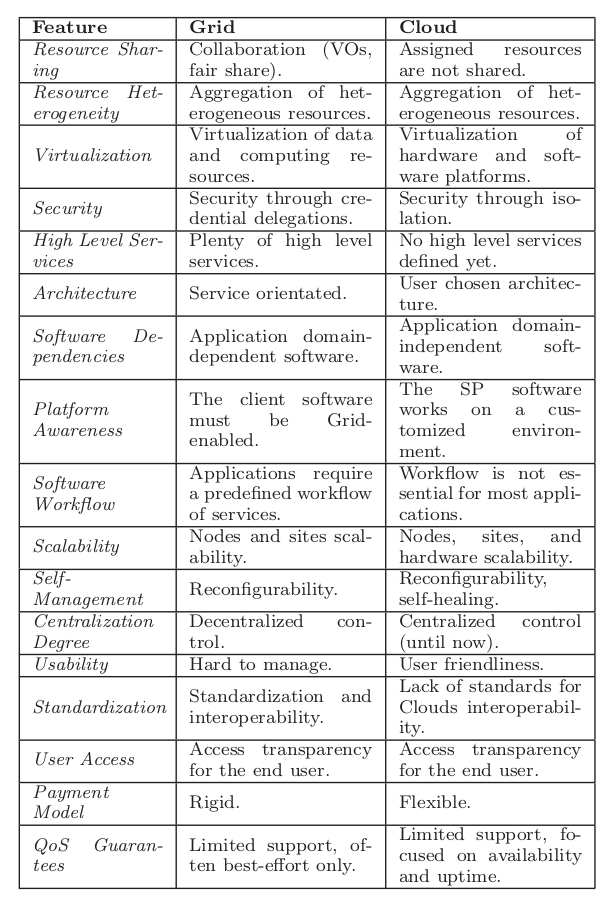
\includegraphics[scale=0.5]{grids_vs_clouds}
    \caption{Comparing Grids and Clouds~\cite{vaquero}.}
    \label{fig:grids_vs_clouds}
  \end{center}
\end{figure}


\chapter{OpenStack VS. OpenNebula} \label{chap:ap2}

\begin{figure}[h!]
  \begin{center}
    \leavevmode 
    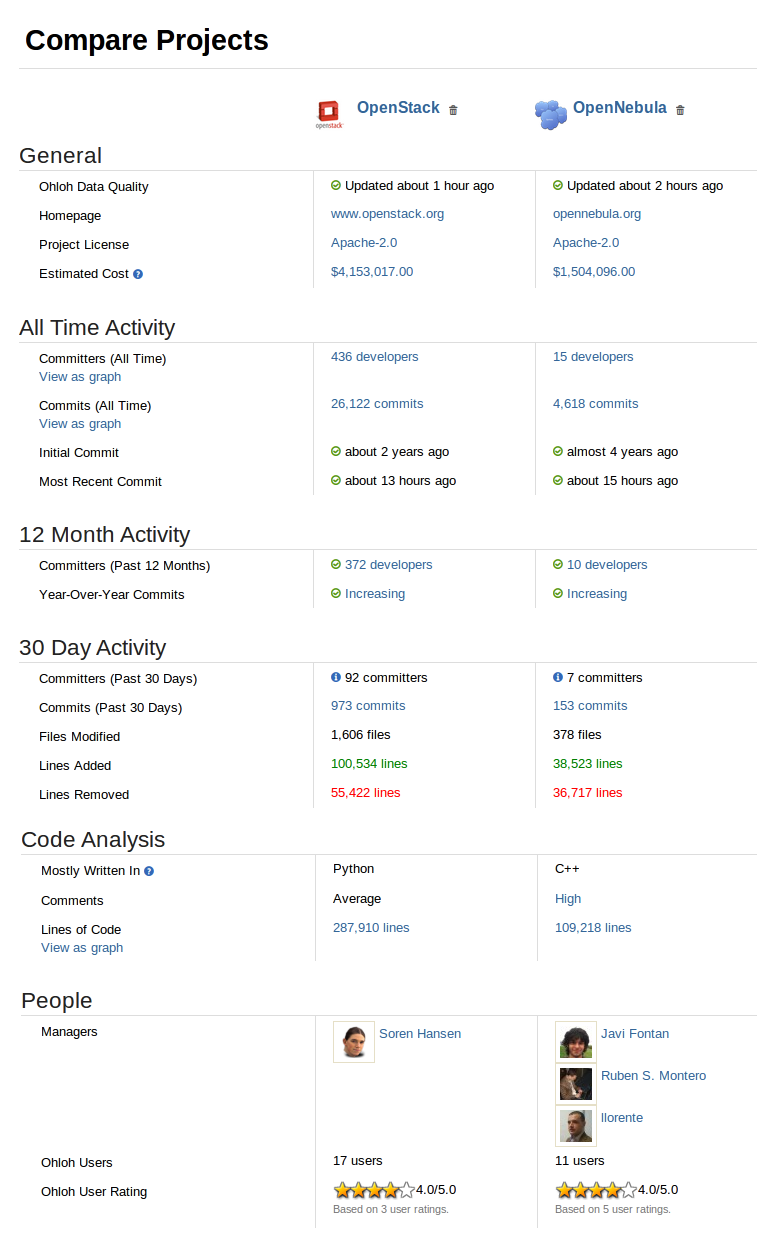
\includegraphics[scale=0.5]{compare}
    \caption{Comparing \textit{OpenStack} and \textit{OpenNebula} on \textit{Ohloh.com}.\cite{ohloh}}
    \label{fig:ohloh_compare}
  \end{center}
\end{figure}

\clearpage

\chapter{IRC conversation about \textit{Cloud-init}} \label{chap:ap3}

Below is presented the IRC conversation on \textit{cloud-init}. Some parts have been left out so that what is important can be understood.

Joshua Harlow uses the alias ``harlowja'', Scott Moser uses the alias ``smoser'' and the author of this report uses the alias ``pteixeira''.

\begin{verse}
{[}03:07{]} {<}pteixeira{>} the way on how different instances from the same images are configured (ip, authentication, etc etc etc)\\
{[}03:08{]} {<}zaitcev{>} So, it's like what Audrey does?\\
{[}03:08{]} {<}pteixeira{>} audrey?\\
{[}03:09{]} {<}zaitcev{>} Actually, I think the fashionable tool these days is cloud-init. Audrey was originally put together by Aeolus people.\\
{[}...{]}\\
{[}03:11{]} {<}pteixeira{>} cloud-init only works on ubuntu based images, right?\\
{[}...{]}\\
{[}03:12{]} {<}smoser{>} coming soon to an RPM based distro near you.\\
{[}03:12{]} {<}smoser{>} (thanks to harlowja and others)\\
{[}...{]}\\
{[}03:12{]} {<}harlowja{>} ya, it will be nicer to work with other distros and debugging and such soon\\
{[}03:12{]} {<}harlowja{>} that is the hope\\
{[}03:12{]} {<}smoser{>} pteixeira, it does exist in fedora at the moment, but in a limited fashion\\
{[}...{]}\\
{[}03:13{]} {<}smoser{>} pteixeira, and there is cloud-init in debian sid right now, although there is work to be don there also.\\
{[}03:13{]} {<}harlowja{>} ya, don't expect it to do to much, i am working on something that abstracts away as much of the distro stuff as possible to helper classes, some stuff won't work  in fedora/rh... ie, aptupgrades and such but those can be removed\\
{[}03:14{]} {<}pteixeira{>} ill use the ubuntu one for now... are there any links that i can follow so i can get some more richness on the document?\\
{[}03:15{]} {<}harlowja{>} code level, or just regular docs, or capability docs?\\
{[}03:15{]} {<}harlowja{>} https://help.ubuntu.com/community/CloudInit\\
{[}03:15{]} {<}harlowja{>} depends on how deep down the rabbit hole u want to go\\
{[}...{]}\\
{[}03:17{]} {<}pteixeira{>} actually, can you link me to the capability docs?\\
{[}03:18{]} {<}harlowja{>} the capabilities, are in that main one, http://bazaar.launchpad.net/~cloud-init-dev/cloud-init/trunk/files/head:/doc/examples/ + code unless there is another better place\\
{[}03:18{]} {<}harlowja{>} i would almost say look at http://bazaar.launchpad.net/~cloud-init-dev/cloud-init/trunk/files/head:/cloudinit/CloudConfig/ also\\
{[}03:18{]} {<}harlowja{>} docs for this kind of stuff could be better i think\\
{[}03:19{]} {<}harlowja{>} datasource* modules there are how data gets loaded\\
{[}03:19{]} {<}harlowja{>} http://bazaar.launchpad.net/~cloud-init-dev/cloud-init/trunk/files/head:/cloudinit/\\
{[}...{]}\\
{[}03:20{]} {<}harlowja{>} http://bazaar.launchpad.net/~harlowja/cloud-init/rework/files might be easier to follow, basically starting in stages.py/init and then to the stages.py/transforms but don't expect that branch to work yet\\
{[}03:20{]} {<}harlowja{>} but for refereence it might be better\\
{[}03:21{]} {<}harlowja{>} sorry, http://bazaar.launchpad.net/~harlowja/cloud-init/rework/files/head:/cloudinit/, not the main dir\\
{[}...{]}\\
{[}03:22{]} {<}smoser{>} almost all of cloudconfig function is documented in the doc/ link or source that harlow pointed at above.\\
{[}03:22{]} {<}smoser{>} and the wiki doc shows what all to feed CloudInit (one of the things you can feed it is cloudconfig).\\
{[}...{]}\\
%{[}03:26{]} {<}pteixeira{>} i want to cite both of you in the thesis, do you guys have any preference on how to do it? :D
%{[}03:26{]} {<}pteixeira{>} preferences*
%{[}03:27{]} {<}harlowja{>} ha, no idear :-p
%{[}03:27{]} {<}harlowja{>} just say 'those awesome dudes on irc'
%{[}03:28{]} {=}{=} dachary {[}~loic@freenode/sponsor/dachary{]} has quit {[}Quit: Leaving.{]}
%{[}03:29{]} {=}{=} dachary {[}~loic@freenode/sponsor/dachary{]} has joined #openstack-dev
%{[}03:31{]} {<}pteixeira{>} ahah ok :D
%{[}03:31{]} {<}pteixeira{>} again, thanks a million for the help :)
\end{verse}

\chapter{vmbuilder script} \label{chap:ap4}

Script used to create VM images dynamically.

This creates a \texttt{KVM Ubuntu} image, version \textit{Precise Pangolin} (\texttt{--suite=precise}), suitable for virtual environments (\texttt{--flavour=virtual}), for 32 bit machine (\texttt{--arch=i386}), using the official \textit{Ubuntu} mirrors to get the packages (\texttt{--mirror}).

The section \texttt{-o --libvirt=qemu:///system} tells the system to register the newly created with the system's virtual machine manager.

In this case, a file named \texttt{vmbuilder.partition} was used to define the disk partitioning. The section \texttt{--templates=templates} points to the folder where \texttt{vmbuilder} should use the templates to build the image. 

After this, we have the definition of the user, the name to be used and the password. This password is reset on first boot, as described in the file \texttt{boot.sh}.

\texttt{--addpkg} tells \texttt{vmbuilder} to install the security updates, \texttt{vim} and \textit{acpid} (used for functions such as closing a laptop lid, pressing the power button, etc).

Finally, \texttt{--mem=256} specifies the total RAM and \textit{--hostname}, defines the machine's hostname.
\begin{verbatim}
#!/bin/bash
sudo vmbuilder kvm ubuntu --suite=precise --flavour=virtual \
	--arch=i386 --mirror=http://de.archive.ubuntu.com/ubuntu \
	-o --libvirt=qemu:///system --ip=192.168.0.101 \
	--part=vmbuilder.partition --templates=templates \
	--user=administrator --name=Administrator --pass=howtoforge \
	--addpkg=vim-nox --addpkg=unattended-upgrades \
	--addpkg=acpid --firstboot=/home/pedro/Desktop/scripts/boot.sh \
	--mem=256 --hostname=vm1 
\end{verbatim}

\chapter{Use cases} \label{chap:ap5}

In this appendix all the use case diagrams are collected.


\begin{figure}[h]
  \begin{center}
    \leavevmode
    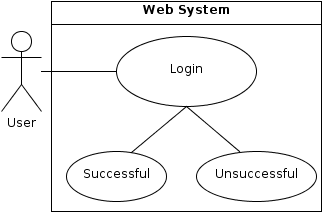
\includegraphics[scale=0.7]{uc/uc1}
    \caption{UC1 -- Login into the web system.}
    \label{fig:uc1}
  \end{center}
\end{figure}

\begin{figure}[h]
  \begin{center}
    \leavevmode
    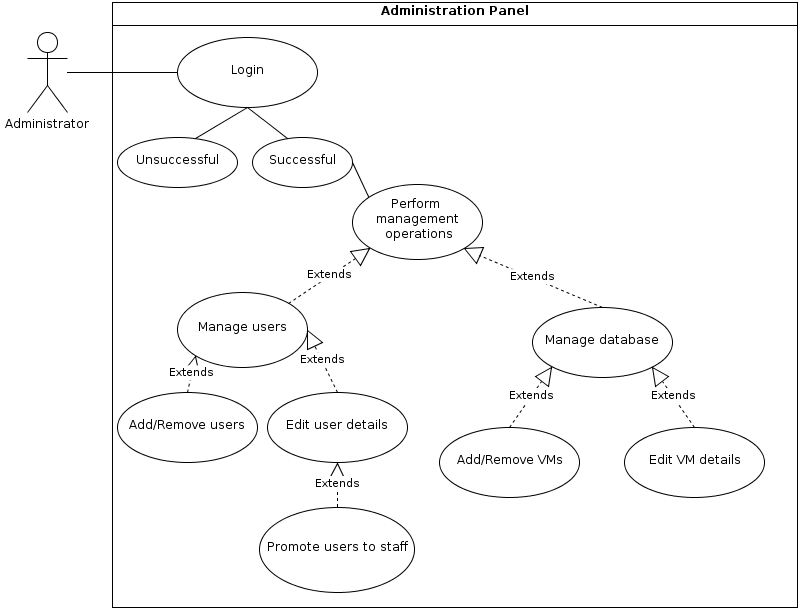
\includegraphics[scale=0.5]{uc/uc2}
    \caption{UC2 -- Perform management operations.}
    \label{fig:uc2}
  \end{center}
\end{figure}


\begin{figure}[h]
  \begin{center}
    \leavevmode
    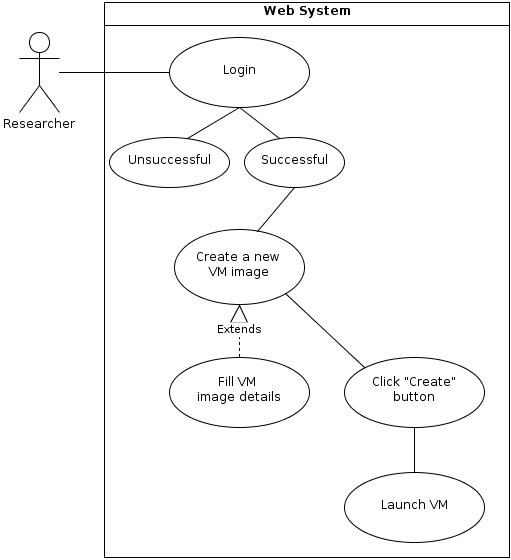
\includegraphics[scale=0.5]{uc/uc3}
    \caption{UC3 -- Create a new VM image.}
    \label{fig:uc3}
  \end{center}
\end{figure}

\begin{figure}[h]
  \begin{center}
    \leavevmode
    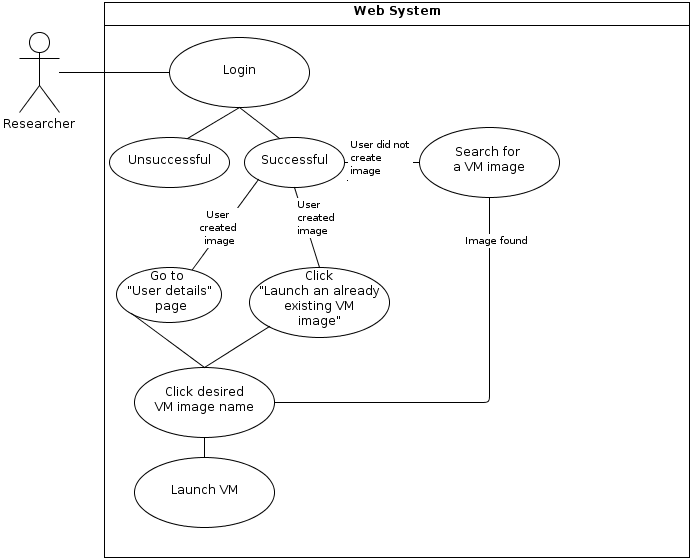
\includegraphics[scale=0.5]{uc/uc4}
    \caption{UC4 -- Launch a VM.}
    \label{fig:uc4}
  \end{center}
\end{figure}

\begin{figure}[h]
  \begin{center}
    \leavevmode
    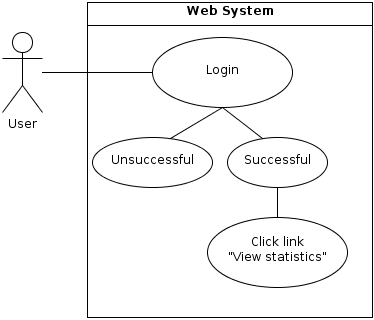
\includegraphics[scale=0.5]{uc/uc5}
    \caption{UC5 -- View system wide statistics.}
    \label{fig:uc5}
  \end{center}
\end{figure}

\begin{figure}[h]
  \begin{center}
    \leavevmode
    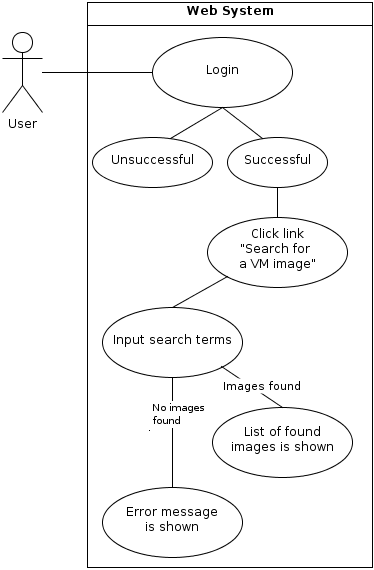
\includegraphics[scale=0.5]{uc/uc6}
    \caption{UC6 -- Search for a VM image.}
    \label{fig:uc6}
  \end{center}
\end{figure}

\begin{figure}[h]
  \begin{center}
    \leavevmode
    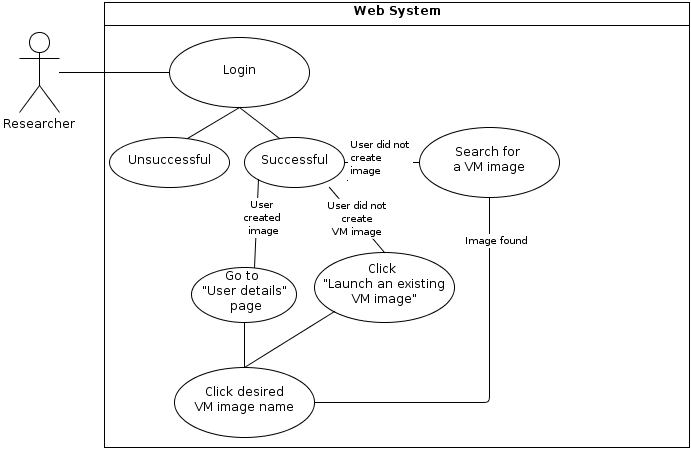
\includegraphics[scale=0.5]{uc/uc7}
    \caption{UC7 -- View the details of an existing VM image.}
    \label{fig:uc7}
  \end{center}
\end{figure}

\begin{figure}[h]
  \begin{center}
    \leavevmode
    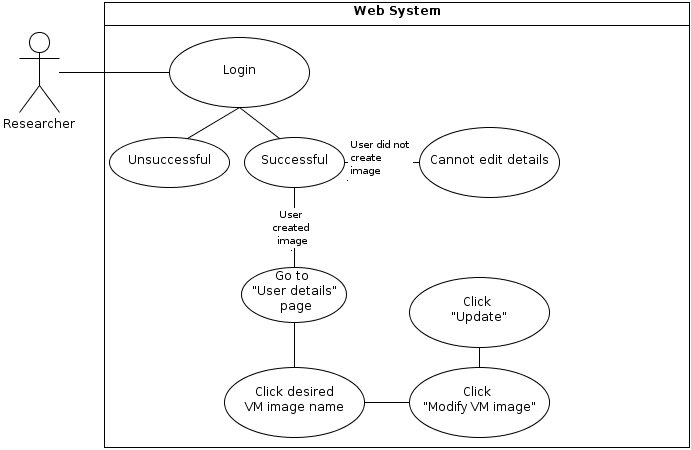
\includegraphics[scale=0.5]{uc/uc8}
    \caption{UC8 -- Modify the details of an existing VM image.}
    \label{fig:uc8}
  \end{center}
\end{figure}

\begin{figure}[h]
  \begin{center}
    \leavevmode
    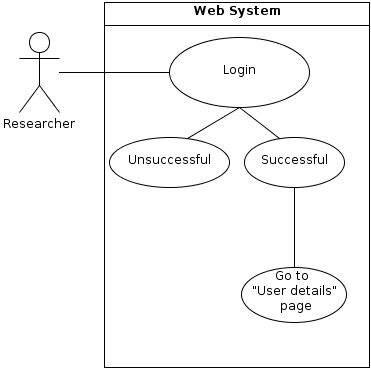
\includegraphics[scale=0.5]{uc/uc9}
    \caption{UC9 -- View user details.}
    \label{fig:uc9}
  \end{center}
\end{figure}

\begin{figure}[h]
  \begin{center}
    \leavevmode
    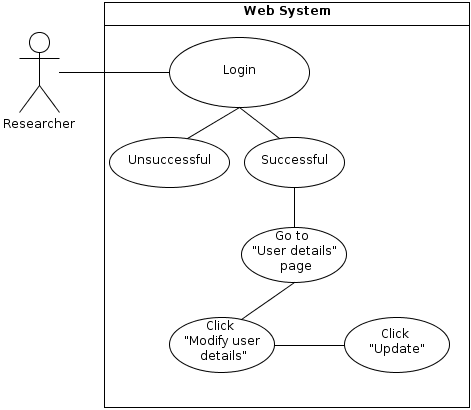
\includegraphics[scale=0.5]{uc/uc10}
    \caption{UC10 -- Modify the user's details.}
    \label{fig:uc10}
  \end{center}
\end{figure}

\begin{figure}[h]
  \begin{center}
    \leavevmode
    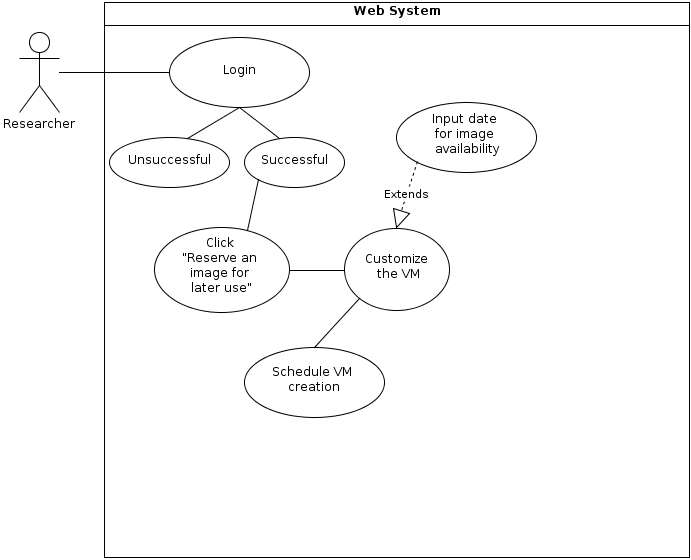
\includegraphics[scale=0.5]{uc/uc11}
    \caption{UC11 -- Reserve an image for later use.}
    \label{fig:uc11}
  \end{center}
\end{figure}

\begin{figure}[h]
  \begin{center}
    \leavevmode
    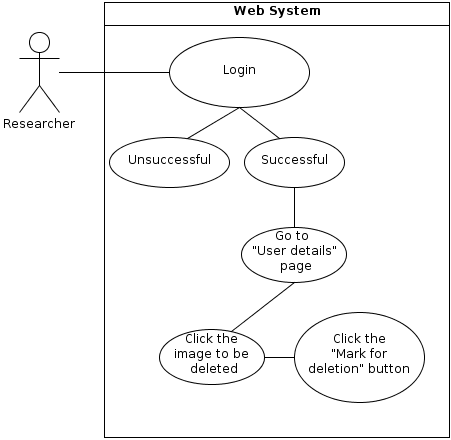
\includegraphics[scale=0.5]{uc/uc12}
    \caption{UC12 -- Mark an image for deletion.}
    \label{fig:uc12}
  \end{center}
\end{figure}

\begin{figure}[h]
  \begin{center}
    \leavevmode
    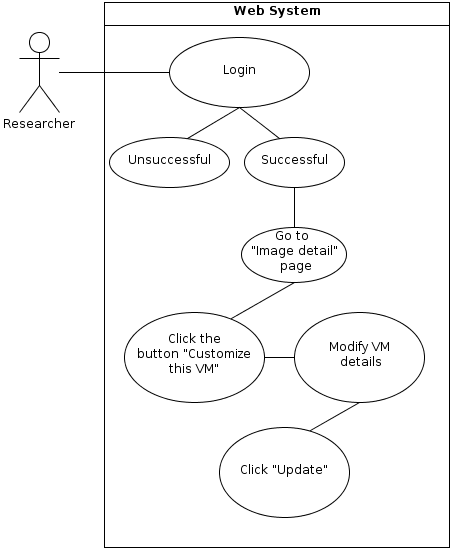
\includegraphics[scale=0.5]{uc/uc13}
    \caption{UC13 -- Customize an image and save it.}
    \label{fig:uc13}
  \end{center}
\end{figure}

\chapter{Web system screenshots} \label{chap:ap6}

In this appendix all the screenshots from the web system are collected.

\begin{figure}[h]
  \begin{center}
    \leavevmode
    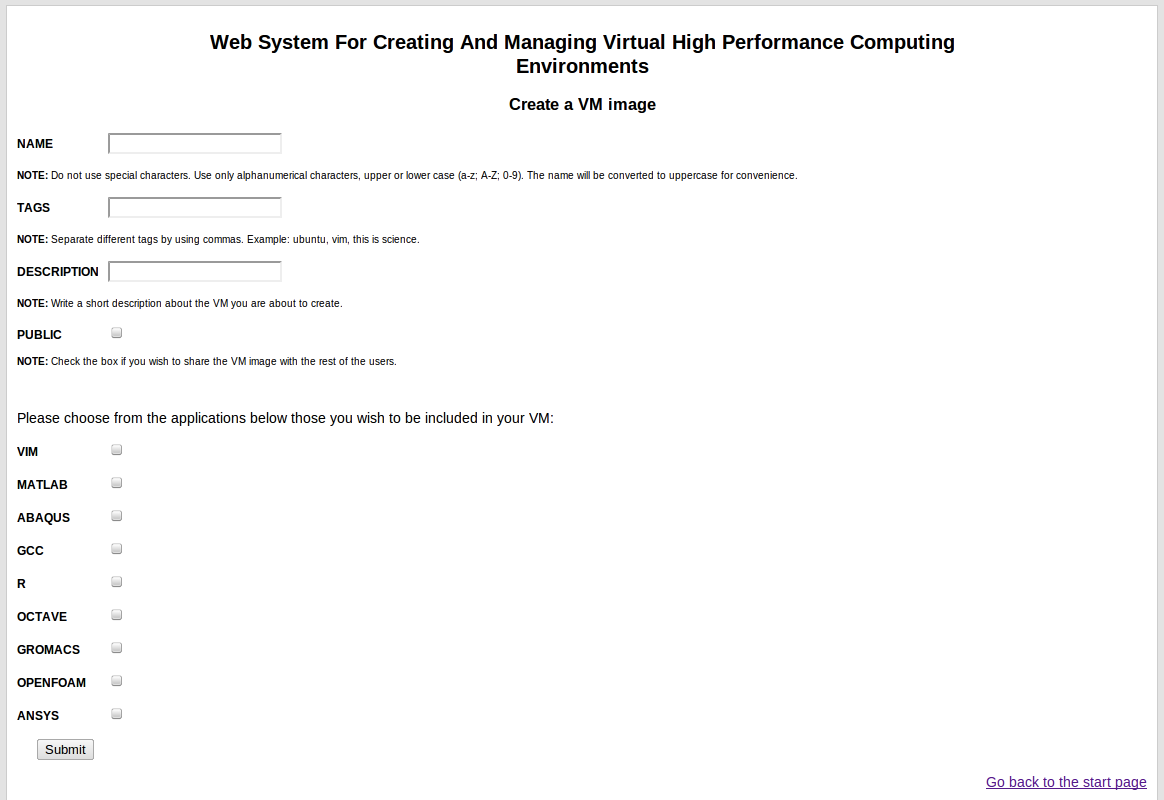
\includegraphics[width=\textwidth]{screenshots/create_image}
    \caption{Create a VM image.}
    \label{fig:vm-creation}
  \end{center}
\end{figure}

\begin{figure}[h]
  \begin{center}
    \leavevmode
    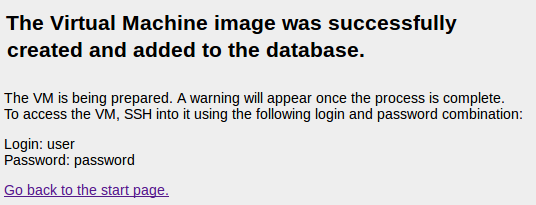
\includegraphics[width=\textwidth]{screenshots/create_results}
    \caption{Post image creation screen.}
    \label{fig:create-results}
  \end{center}
\end{figure}


\begin{figure}[h]
  \begin{center}
    \leavevmode
    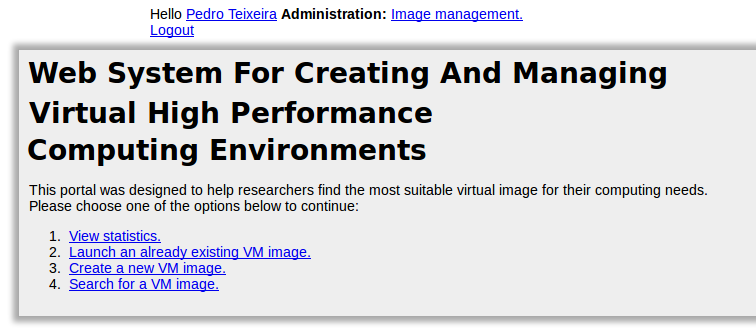
\includegraphics[width=\textwidth]{screenshots/index}
    \caption{The start page.}
    \label{fig:index}
  \end{center}
\end{figure}

\begin{figure}[h]
  \begin{center}
    \leavevmode
    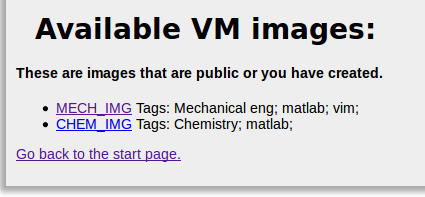
\includegraphics[scale=0.8]{screenshots/list_vms}
    \caption{List of available VMs to launch.}
    \label{fig:available-vms}
  \end{center}
\end{figure}

\begin{figure}[h]
  \begin{center}
    \leavevmode
    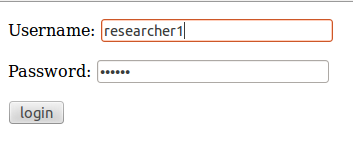
\includegraphics[scale=0.5]{screenshots/login}
    \caption{Login screen.}
    \label{fig:login}
  \end{center}
\end{figure}

\begin{figure}[h]
  \begin{center}
    \leavevmode
    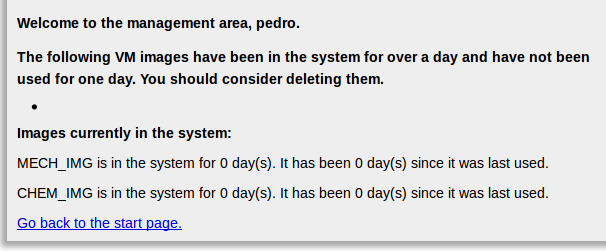
\includegraphics[width=\textwidth]{screenshots/management}
    \caption{Management area accessible from the start page.}
    \label{fig:management}
  \end{center}
\end{figure}

\begin{figure}[h]
  \begin{center}
    \leavevmode
    
\includegraphics{screenshots/search}
    \caption{Search page.}
    \label{fig:search-page}
  \end{center}
\end{figure}

\begin{figure}[h]
  \begin{center}
    \leavevmode
    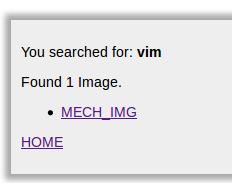
\includegraphics{screenshots/search_results}
    \caption{Results of a search for ``vim''.}
    \label{fig:search-results}
  \end{center}
\end{figure}

\begin{figure}[h]
  \begin{center}
    \leavevmode
    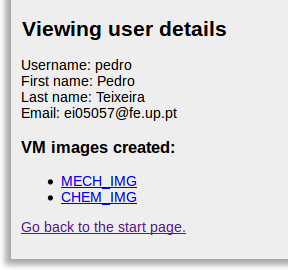
\includegraphics{screenshots/user_details}
    \caption{User details page.}
    \label{fig:1}
  \end{center}
\end{figure}

\begin{figure}[h]
  \begin{center}
    \leavevmode
    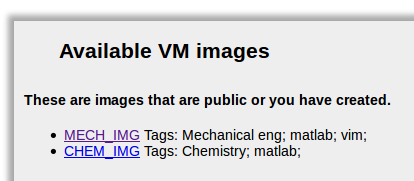
\includegraphics{screenshots/statistics1}
    \caption{VM images available to the user (includes public and created by the user).}
    \label{fig:user-vms}
  \end{center}
\end{figure}

\begin{figure}[h]
  \begin{center}
    \leavevmode
    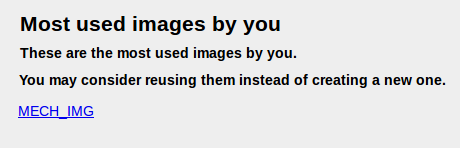
\includegraphics[width=\textwidth]{screenshots/statistics2}
    \caption{Most used VM images by the current user.}
    \label{fig:user-mostused-vms}
  \end{center}
\end{figure}

\begin{figure}[h]
  \begin{center}
    \leavevmode
    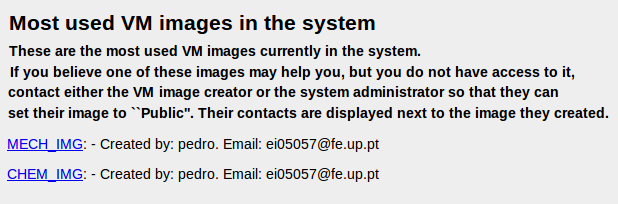
\includegraphics[width=\textwidth]{screenshots/statistics3}
    \caption{Most used VM images system wide.}
    \label{fig:system-mostused-vms}
  \end{center}
\end{figure}

\begin{figure}[h]
  \begin{center}
    \leavevmode
    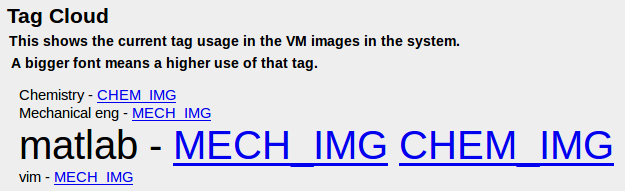
\includegraphics[width=\textwidth]{screenshots/statistics4}
    \caption{Tag cloud.}
    \label{fig:tagcloud}
  \end{center}
\end{figure}

\begin{figure}[h]
  \begin{center}
    \leavevmode
    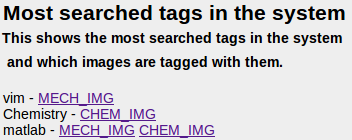
\includegraphics{screenshots/statistics5}
    \caption{Most searched ``tags'' in the system.}
    \label{fig:mostsearched-tags}
  \end{center}
\end{figure}

\begin{figure}[h]
  \begin{center}
    \leavevmode
    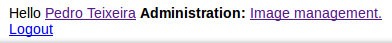
\includegraphics{screenshots/management-login}
    \caption{Link to ``Image management''.}
    \label{fig:management-login}
  \end{center}
\end{figure}

%%----------------------------------------
%% Final materials
%%----------------------------------------

%% Bibliography
%% Comment the next command if BibTeX file not used
%% bibliography is in ``myrefs.bib''
\PrintBib{myrefs}

%% Index
%% Uncomment next command if index is required
%% don't forget to run ``makeindex thesis'' command
%\PrintIndex

\end{document}
